% CVPR 2027 submission draft, built on the official CVPR author kit
% (github.com/cvpr-org/author-kit, main @ 2917585, the CVPR 2026 kit; no 2027 kit exists yet).
%
% Every number in the text carries a trailing comment "% src: <file>" naming the result
% file it was copied from. Paths are relative to the project root (the folder holding docs/ and work/).
% Numbers marked "derived" were recomputed from score parquets by paper/scripts/derive_numbers.py,
% whose log (paper/data/derive_numbers.log) shows every cross-check against the original reports.

\documentclass[10pt,twocolumn,letterpaper]{article}

%%%%%%%%% PAPER TYPE
% \usepackage{cvpr}              % camera-ready
\usepackage[review]{cvpr}        % review (anonymous) version
% \usepackage[pagenumbers]{cvpr} % arXiv version

%% This file contains a number of tweaks that are typically applied to the main document.
%% They are not enabled by default, but can be enabled by uncommenting the relevant lines.


%%
%% Official support for 2-column teaser figure
%%
\usepackage{cuted} %< for strip environment

%%
%% For auto-referencing of figures (see fig/teaser.tex and \label{} therein) 
%%
\usepackage{currfile} %< for \currfilebase macro

%%
%% caption and (global) spacing overrides
%%
\usepackage{caption} %< for "\captionof" commands (teaser)
% \setlength{\abovecaptionskip}{.5em} % space above caption
% \setlength{\belowcaptionskip}{1em} % space below caption

%%
%% Inline annotations; for predefined colors, refer to "dvipsnames" in the xcolor package:
%% https://tinyurl.com/overleaf-colors
%%
\newcommand{\red}[1]{{\color{red}#1}}
\newcommand{\todo}[1]{{\color{red}#1}}
\newcommand{\TODO}[1]{\textbf{\color{red}[TODO: #1]}}
%%
%% Disable for camera ready / submission by uncommenting these lines:
%%
% \renewcommand{\TODO}[1]{}
% \renewcommand{\todo}[1]{#1}

%%
%% Work harder in optimizing text layout. Typically shrinks text by 1/6 of page, enable
%% it at the very end of the writing process, when you are just above the page limit.
%%
% \usepackage{microtype}

%%
%% Fine-tune paragraph spacing.
%%
% \renewcommand{\paragraph}[1]{\vspace{.5em}\noindent\textbf{#1.}}

%%
%% Globally adjusts space between figure and caption.
%%
% \setlength{\abovecaptionskip}{.5em}

%%
%% Allows "the use of \paper to refer to the project name"
%% with automatic management of space at the end of the word.
%%
% \usepackage{xspace}
% \newcommand{\paper}{ProjectName\xspace}

%%
%% Commonly used math definitions.
%%
% \DeclareMathOperator*{\argmin}{arg\,min}
% \DeclareMathOperator*{\argmax}{arg\,max}

%%
%% Tighten underline.
%%
% \usepackage{soul}
% \setuldepth{foobar}

%%
%% Reconfigure paragraph (tweaks spacing)
%%

%% Project macros (kept out of the kit's preamble.tex).

\usepackage{multirow}
\usepackage{pifont}
\usepackage{array}

%% Dataset name. "MedForensics" is taken (MICCAI 2025); candidates are listed in README.md.
\newcommand{\dataset}{NullTwin-Med\xspace}

%% Anonymous-link placeholder. Do not replace with a real URL before decisions:
%% CVPR forbids links that identify the authors or expand the paper's content.
\newcommand{\anonlink}{\texttt{[anonymous link withheld for review]}\xspace}

%% Teaser: \teaserdrafttrue shows figures/teaser_draft.pdf (built from our own release
%% images by scripts/make_figures.py); \teaserdraftfalse shows the placeholder box.
\newif\ifteaserdraft
\teaserdraftfalse

\newcommand{\cmark}{\ding{51}}
\newcommand{\xmark}{\ding{55}}
\newcommand{\na}{--}

%% Visible draft markers. Comment the two lines in preamble.tex before submission.
\newcommand{\PENDING}[1]{\textbf{\color{orange}[PENDING: #1]}}


\definecolor{cvprblue}{rgb}{0.21,0.49,0.74}
\usepackage[pagebackref,breaklinks,colorlinks,allcolors=cvprblue]{hyperref}

%%%%%%%%% PAPER ID
\def\paperID{*****} % enter the OpenReview paper ID here
\def\confName{CVPR}
\def\confYear{2027}

%%%%%%%%% TITLE
\title{\dataset: Null Twins Show That Medical Forgery Detectors\\Respond to the Autoencoder, Not the Edit}

%%%%%%%%% AUTHORS (anonymous for review)
\author{Anonymous CVPR submission\\
Paper ID \paperID}

\begin{document}
\maketitle
\begin{strip}
\centering
\ifteaserdraft
  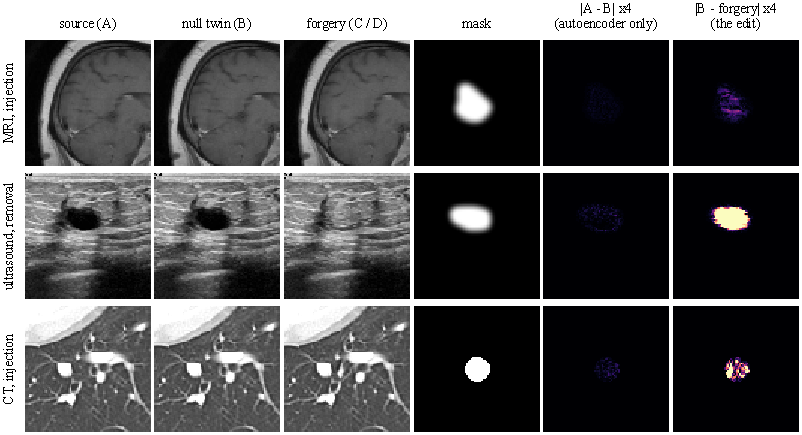
\includegraphics[width=\linewidth]{figures/teaser_draft.pdf}
\else
  \fbox{\parbox[c][1.55in][c]{0.97\linewidth}{\centering\small
  \textbf{[TEASER PLACEHOLDER]}\\[3pt]
  Three lineages (MRI injection, ultrasound removal, CT injection), one row each, cropped around the mask.
  Columns: \emph{source} (A) \textbar{} \emph{null twin} (B: the source round-tripped through the SD autoencoder inside the mask, no edit) \textbar{}
  \emph{forgery} (C or D) \textbar{} \emph{mask} \textbar{} $|$A$-$B$|\times4$ (what the autoencoder alone changed) \textbar{} $|$B$-$forgery$|\times4$ (what the edit changed).\\[3pt]
  Message: the autoencoder change is nearly invisible, the edit is not, yet a standard detector calls both images fake.
  Annotate each image with MedForge-Reasoner's or standard Mesorch's verdict once a per-image score is chosen.\\[3pt]
  A draft built from our own release images is in \texttt{figures/teaser\_draft.pdf}; set \texttt{\textbackslash teaserdrafttrue} in \texttt{macros.tex} to show it.
  No MedForge image may appear (C-UDA licence).}}
\fi
\captionsetup{hypcap=false}
\captionof{figure}{\textbf{One lineage, three images.} The null twin (B) went through the generator's autoencoder exactly as the forgery did but contains no edit; outside the mask, every image is bit-identical to the source.
MedForge-Reasoner flags 0.5\% of untouched scans % src: paper/data/medforge_reasoner_hardlabel.csv (derived from work/e0/out_local/e2/scores_reasoner.parquet)
and 92.5\% of their SD-autoencoder twins as deepfakes (\cref{sec:confound}). % src: paper/data/medforge_reasoner_hardlabel.csv
\TODO{replace placeholder with the final teaser}}
\captionsetup{hypcap=true}
\label{fig:teaser}
\end{strip}

\begin{abstract}
Medical image forgery detectors are trained and tested on one question: is this scan untouched or edited?
A generative edit, however, changes a scan in two ways at once.
It inserts or removes a lesion, and it passes the image through the generator's autoencoder.
We show that medical forgery detectors, including MedForge's own, respond to the autoencoder processing rather than to the edit.
MedForge-Reasoner calls 0.5\% of untouched scans fake, % src: paper/data/medforge_reasoner_hardlabel.csv (derived from work/e0/out_local/e2/scores_reasoner.parquet)
but 92.5\% of the same scans after they are passed, unedited, through Stable Diffusion's autoencoder, % src: paper/data/medforge_reasoner_hardlabel.csv
and on 22 of 30 normal scans it draws a lesion-sized box around a manipulation that does not exist. % src: docs/council/round3/experiments/local/r3_box_audit_normals.csv; R3_STEP1_REPORT.md (Sec. 1)
On our data, a fine-tuned Mesorch separates untouched images from forgeries at AUC 0.963, % src: work/e0/out_local/tables/table_main.csv
but forgeries from unedited images passed through the same autoencoder at only 0.536. % src: work/e0/out_local/tables/table_main.csv
To make this measurable we release \dataset, a six-modality benchmark of 3,956 source images with local lesion injections and removals. % src: docs/council/context_dossier.md (A)
Every generative edit comes with a per-pixel lesion mask, a background bit-identical to the source, and an unedited image passed through the generator's autoencoder, over three generators, one of them held out.
Its protocol scores each detector at a single operating point, fixed on a calibration split, against every kind of unedited image, per modality.
No detector we test wins everywhere.
At 95\% recall, fine-tuned single-image detectors flag 93--94\% of unedited autoencoder images, % src: docs/council/round3/experiments/local/r3_operating_points.csv (V0, V1, fpr_cal_SD_null)
and a zero-parameter comparison against a reference image, despite an AUC of 0.921, flags 44\% of them and 98--99\% of images re-encoded by an autoencoder. % src: docs/council/round3/experiments/local/r3_operating_points.csv (sub_raw: fpr_cal_SD_null, fpr_vqvae, fpr_sdxlvae); work/e0/out_local/e0x/e0a/e0a_deltas.csv
\end{abstract}

\section{Introduction}
\label{sec:intro}

Tampering with medical images is a demonstrated threat.
In the CT-GAN study, lung nodules injected into or removed from CT scans fooled radiologists in 99\% and 94\% of cases~\cite{mirsky2019ctgan}. % src: docs/council/context_dossier.md (G, CT-GAN row)
Text-guided editors now make such edits easy across modalities~\cite{medbanana2025,chen2026medforge}, and detecting them has become an active benchmark area~\cite{zingarini2024m3dsynth,grabovski2025btd,li2025medforensics,chen2026medforge}.

These benchmarks score a detector by how well it separates untouched images from edited ones.
But a generative edit is two interventions, not one.
A lesion is painted inside a mask, and the image (or a crop of it) is encoded and decoded by the generator's autoencoder.
In existing medical corpora the untouched class never passes through that autoencoder, so a detector can score well by recognising the autoencoder and never looking at the lesion.
For natural images this shortcut is known, and it has been turned into better training data: Aligned Datasets~\cite{rajan2025aligned} trains on autoencoder reconstructions of real images, B-Free~\cite{guillaro2025bfree} on self-conditioned inpaintings with the background restored, and INP-X~\cite{nebioglu2026inpx} shows that detection rates fall from over 91\% to about 55\% once the inpainted image's background is restored. % src: docs/council/round2/irp_prior_art.md (Controls and threat model)
No medical forgery benchmark controls for it.

Whether autoencoder processing alone should count as forgery depends on the definition.
Under a provenance definition, where any image a generative model has touched is synthetic, it should.
We adopt CT-GAN's tamper definition instead~\cite{mirsky2019ctgan}: a forgery is content changed between the scanner and the archive.
Under that definition, an image that passed an autoencoder unedited is authentic, and a provenance detector cannot tell a malicious edit from benign neural processing.

We find that medical forgery detectors, including MedForge's own, respond to autoencoder processing rather than to the edit.
MedForge-Reasoner~\cite{chen2026medforge}, an open-weight detector trained on MedForge-90K, flags all 48 MedForge forgeries we sampled % src: paper/data/medforge_reasoner_hardlabel.csv
and 0.5\% of 186 untouched MedForge test scans. % src: paper/data/medforge_reasoner_hardlabel.csv
After those scans pass through the Stable Diffusion inpainting autoencoder with no edit, it flags 95.8\% of brain MRI and 88.9\% of fundus scans (\cref{fig:medforge}). % src: docs/council/round3/experiments/local/r3_box_audit.csv (N_sd, real, fake_rate)
It is wrong under either definition: every one of those verdicts comes with a lesion-sized box, comparable in size to the boxes it draws on real MedForge forgeries, whereas an image that is synthetic as a whole would call for a whole-image box (\cref{sec:confound}). % src: docs/council/round3/experiments/local/R3_STEP1_REPORT.md (Sec. 1: every null-twin fake call has a box)
The same holds for conventionally trained detectors on our own data.
Mesorch~\cite{zhu2025mesorch} fine-tuned to separate sources from forgeries scores AUC 0.963 on that task % src: work/e0/out_local/tables/table_main.csv
but 0.536 when the negatives are the forgeries' own null twins, % src: work/e0/out_local/tables/table_main.csv
images that passed the same autoencoder without being edited.
By our fingerprint-share metric (\cref{sec:protocol}), 93\% of its margin over chance is reproduced by an image nobody edited. % src: paper/data/fingerprint_share_test.csv (derived); work/e0/out_local/tables/E1_REPORT.md

To make this measurable, we release \dataset.
To our knowledge, it is the first publicly released multi-modality medical local-edit forgery benchmark that pairs every generative edit with a per-pixel (non-box) mask, a background bit-identical to the source, and an autoencoder-matched null twin that passes the same generator without an edit.
Each \emph{lineage} is one source image with one mask and one random seed, from which every other image is derived: the source itself, a \emph{null twin} per generator (the source passed through that generator's autoencoder inside the mask, with nothing edited), the lesion injection or removal, and two copy-move controls.
\dataset holds 3,956 lineages across CT, endoscopy, histopathology, MRI, ultrasound and X-ray, % src: docs/council/context_dossier.md (A)
edited by Stable Diffusion~1.5 inpainting and big-LaMa, with SDXL inpainting held out as a third generator.

AUC alone cannot rank detectors on \dataset, so the protocol fixes one operating point on calibration and reads it against every kind of unedited image.
Measured this way, single-image detection falls from 0.963 on the conventional task % src: work/e0/out_local/tables/table_main.csv
to at most 0.768 against the twin, and stays near chance on CT. % src: work/e0/out_local/tables/e9_final_comparison.csv
Comparing with the null twin as a reference makes AUC easy, but not the operating point.
A zero-parameter pixel subtraction reaches 0.921, % src: work/e0/out_local/e0x/e0a/e0a_deltas.csv
or 0.976 when standardised per modality, % src: docs/council/round3/experiments/local/r3_subtraction_standardised.csv (standardised, ALL)
which is within 0.008 of a learned FC-Siam-diff baseline~\cite{daudt2018fcsiam}; % src: docs/council/round3/experiments/local/r3_subtraction_gap_to_p1n.csv (standardised, ALL)
yet at 95\% recall subtraction flags 47\% of test null twins, % src: docs/council/round3/experiments/local/r3_operating_points.csv (sub_raw, fpr_test_SD_null)
and the learned baseline flags 78\% of denoised sources. % src: docs/council/round3/experiments/local/r3_operating_points.csv (p1n, fpr_nlmeans)
No detector we test is acceptable on every negative type.
Our contributions are:
\begin{itemize}[leftmargin=*,itemsep=1pt,topsep=2pt]
\item \textbf{Dataset.} \dataset, a six-modality local-edit benchmark with per-pixel lesion-shaped masks, bit-identical backgrounds and an autoencoder-matched null twin for every generative edit, over three generators with one held out (\cref{sec:dataset}).
\item \textbf{Protocol.} Four controls that make a forgery-detection number interpretable: an autoencoder-matched unedited twin for every edit; one calibration operating point scored against every negative type, per modality, with same-generator drift beside cross-generator transfer; null-penalised localisation F1; and a mask-shape baseline beside every removal number. These come with frozen leak-free splits and calibration-only selection (\cref{sec:protocol}).
\item \textbf{Findings.} The autoencoder response in three settings, including MedForge's own detector; per-modality operating points for single-image and reference-based detectors, which show that AUC gains do not carry over to false-alarm rates; and an oracle-mask diagnostic separating finding an edit from judging it (\cref{sec:results}).
\end{itemize}

\section{Related work}
\label{sec:related}

\begin{table*}[t]
\centering
\caption{\textbf{Medical forgery datasets.} ``n.s.'': not stated in the paper or card; ``n/a'': not applicable (whole images are synthesised). \emph{Null twin}: an unedited copy that passed the same generator. \emph{Background preserved}: pixels outside the edit are bit-identical to the source. Public status checked on 29 Sep 2026. % src: docs/council/round2/landscape_and_odds.md (Sec. 2)
}
\label{tab:datasets}
\footnotesize
\setlength{\tabcolsep}{3.0pt}
\begin{tabular}{@{}llllllccl@{}}
\toprule
Dataset & Venue & Modalities & Size & Edits & Mask & Null twin & Bkgd.\ preserved & Public \\
\midrule
CT-GAN~\cite{mirsky2019ctgan} & USENIX Sec 2019 & 3D lung CT & 100 scans & inject / remove & location only & \xmark & n.s. & \cmark \\ % src: docs/council/round2/landscape_and_odds.md (Sec. 2)
M3Dsynth~\cite{zingarini2024m3dsynth} & ICASSP 2024 & 3D lung CT & 8,577 scans & inject / remove & 32\,mm cube & \xmark & n.s. & \cmark\ (non-profit) \\ % src: docs/council/round2/landscape_and_odds.md (Sec. 2)
BTD test sets~\cite{grabovski2025btd} & TIST 2025 & lung CT, breast MRI & 6 test sets & inject / remove & n.s. & \xmark & n.s. & \cmark \\ % src: docs/council/round2/landscape_and_odds.md (Sec. 2)
MedForensics~\cite{li2025medforensics} & MICCAI 2025 & 6 modalities & 116K (256$^2$) & full synthesis & image label & \xmark & n/a & not released$^{\dagger}$ \\ % src: docs/council/round2/landscape_and_odds.md (Sec. 2)
CTForensics~\cite{ctforensics2026} & arXiv 2026 & 2D CT & 75,990 & full synthesis & image label & \xmark & n/a & not yet \\ % src: docs/council/round2/landscape_and_odds.md (Sec. 2)
Med-Banana-50K~\cite{medbanana2025} & arXiv 2025 & CXR, brain MRI, fundus & 50,635 edits & semantic edits & n.s. & \xmark & n.s. & \cmark \\ % src: docs/council/round2/landscape_and_odds.md (Sec. 2)
MedForge-90K~\cite{chen2026medforge} & ACL 2026 & CXR, brain MRI, fundus & 95,276 & semantic edits, 10 editors & boxes & \xmark & \xmark & \cmark\ (C-UDA) \\ % src: docs/council/round2/landscape_and_odds.md (Sec. 1, 2)
\midrule
\dataset (ours) & -- & CT, endo., histo., MRI, US, X-ray & 3,956 lineages & inject / remove, copy-move & per-pixel, lesion-shaped & \cmark & \cmark\ (100\%) & \cmark$^{\ddagger}$ \\ % src: docs/council/context_dossier.md (A); docs/MEDFORENSICS_V2.md (Sec. 8.6, audit 4.1)
\bottomrule
\end{tabular}\\[2pt]
\begin{minipage}{\linewidth}\footnotesize
$^{\dagger}$The paper's MICCAI rebuttal states that the dataset and code will be released upon acceptance~\cite{li2025medforensics}; we found no public release by 29 Sep 2026. % src: docs/council/round2/landscape_and_odds.md (Sec. 2, [R7]); papers.miccai.org/miccai-2025/0935-Paper2888.html (rebuttal)
$^{\ddagger}$Gated access; a subset, loader and datasheet are in the supplementary material, and the full release is public by camera-ready (\anonlink).
\end{minipage}
\end{table*}

\paragraph{Generator fingerprints and how to control them.}
Real-versus-fake detectors read low-level generator traces: up-sampling artefacts (NPR~\cite{tan2024npr}), reconstruction error under a diffusion model (DIRE~\cite{wang2023dire}, LaRE$^2$~\cite{luo2024lare2}) or its autoencoder (AEROBLADE~\cite{ricker2024aeroblade}), or frozen CLIP features (UniFD~\cite{ojha2023unifd}).
Inpainting detectors such as End4~\cite{wang2025end4} and HIDE~\cite{ji2026hide} reuse one-step denoising or diffusion features, and training-free localisation compares guided diffusion reconstructions~\cite{zhang2025trainingfree}; HIDE falls from AUC 0.98 on SD-1.5 inpaintings to 0.57 on SD-2. % src: docs/council/round2/irp_prior_art.md (Local diffusion forensics)
Image manipulation localisation models (TruFor~\cite{guillaro2023trufor}, MVSS-Net~\cite{chen2021mvss}, PSCC-Net~\cite{liu2022pscc}, IML-ViT~\cite{ma2023imlvit}, Mesorch~\cite{zhu2025mesorch}; benchmarked in IMDL-BenCo~\cite{ma2024imdlbenco}) predict a per-pixel map.
Three works confront the fingerprint in natural images.
Aligned Datasets~\cite{rajan2025aligned} uses autoencoder reconstructions of real images, without denoising, as the fake class, the same object as our null twin.
B-Free~\cite{guillaro2025bfree} generates fakes by self-conditioned inpainting and adds local inpaintings with the original background restored.
INP-X~\cite{nebioglu2026inpx} shows that detectors rely on global artefacts and collapse when the background is restored.
The first two use aligned images as \emph{training data}, and the third as a stress test, all for whole-image detection of natural images.
We use the twin as a \emph{measurement control} for local medical edits: every forgery ships with its twin, so the share of a detector's score that the autoencoder explains can be read off directly.

\paragraph{Medical forgery data.}
\Cref{tab:datasets} lists the medical datasets.
CT-GAN~\cite{mirsky2019ctgan}, M3Dsynth~\cite{zingarini2024m3dsynth} and BTD~\cite{grabovski2025btd} inject and remove lung nodules in 3D CT; MedForensics~\cite{li2025medforensics} and CTForensics~\cite{ctforensics2026} target fully synthetic images.
MedForge-90K~\cite{chen2026medforge} is the closest and largest local-edit benchmark: 95,276 images over three modalities and ten editors, % src: docs/council/round2/landscape_and_odds.md (Sec. 1)
localised by boxes, with the editor's whole output saved, so the background also changes. % src: docs/council/round2/landscape_and_odds.md (Sec. 1); docs/council/round2/experiments/README.md (harness fact 6)
None has a null twin.
Our contribution is not scale: \dataset trades MedForge's breadth for the control that makes its numbers interpretable, and we use MedForge itself as a test bed (\cref{sec:confound}).

\paragraph{Anomaly detection and reconstruction.}
Predicting a clean image and reading the residual is the anomaly-detection recipe: DRAEM~\cite{zavrtanik2021draem} and RIAD~\cite{zavrtanik2021riad} reconstruct or inpaint, pDDPM~\cite{behrendt2024pddpm} denoises patches at a fixed timestep, and LMD~\cite{liu2023lmd} inpaints under alternating masks.
Applied to forgeries, these priors meet a medical complication: real pathology is itself an anomaly, so a model trained on healthy tissue can score an unedited lesion above the healthy tissue painted over it.
A frozen-generator probe from this family is at chance on \dataset (\cref{sec:oracle}).

\paragraph{Change detection and integrity checks.}
When a reference image exists, for example an archived original, tamper detection becomes change detection.
FC-Siam-diff~\cite{daudt2018fcsiam}, BIT~\cite{chen2022bit} and ChangeFormer~\cite{bandara2022changeformer} compare two images with a shared encoder, and robust image hashing~\cite{venkatesan2000hash,swaminathan2006hash} certifies that content is unchanged under benign processing.
Our reference-based rows are baselines from these families (FC-Siam-diff on a Mesorch trunk, subtraction, a block-wise hash), and none is claimed as new; their role is to show what the protocol's operating points reveal.
For small targets, tiled inference (SAHI~\cite{akyon2022sahi}) is the standard remedy; CT lesions in \dataset cover about 0.1\% of the frame. % src: docs/council/context_dossier.md (A, mask areas)

\section{The \dataset benchmark}
\label{sec:dataset}

\paragraph{Lineages and image variants.}
A \emph{lineage} is one source image, one mask and one random seed.
Every other image in the lineage is derived from the source with that mask and seed, and differs from it only inside the feathered mask.
We use five letters throughout.
\textbf{A}, the \emph{source}, is the untouched image.
\textbf{B}, the \emph{null twin}, is the source passed through a generator's autoencoder inside the mask with nothing edited; there is one per generator (B$_\text{SD}$, B$_\text{LaMa}$, B$_\text{SDXL}$).
\textbf{C}, an \emph{injection}, paints a lesion into healthy tissue.
\textbf{D}, a \emph{removal}, paints healthy tissue over a real, human-outlined lesion.
\textbf{CM}, a \emph{copy-move}, moves tissue within the same image, by translation or with a 3--15$^\circ$ rotation; % src: docs/council/context_dossier.md (arm glossary)
no generator is involved, so copy-move is the generator-free control.
Injection lineages contain A, B and C, removal lineages A, B and D, and all lineages contain CM.
\dataset has 2,677 injection and 1,279 removal lineages. % src: docs/council/context_dossier.md (A, Arms)

\paragraph{Sources and masks.}
CT contributes 900 lineages, % src: docs/council/context_dossier.md (A); Deepfakedoctillnow.pdf p.1
rendered in a lung window at 512$^2$ from LIDC-IDRI~\cite{armato2011lidc} (1,018 series, 1,010 patients). % src: docs/MEDFORENSICS_V2.md (Sec. 3)
CT injections use slices that none of the four LIDC readers annotated, so the tissue at the edit is verified healthy; CT removals use nodule slices with a unanimous four-reader contour, dilated by 3\,px. % src: docs/MEDFORENSICS_V2.md (Sec. 3)
Endoscopy (830 lineages) % src: docs/council/context_dossier.md (A, lineages by modality)
uses HyperKvasir~\cite{borgli2020hyperkvasir} frames for injection and Kvasir-SEG~\cite{jha2020kvasirseg} polyps for removal.
Histopathology (427) % src: docs/council/context_dossier.md (A, lineages by modality)
uses LC25000 colon tiles~\cite{borkowski2019lc25000}.
MRI (754) % src: docs/council/context_dossier.md (A, lineages by modality)
uses a public brain-tumour aggregate~\cite{nickparvar2021brainmri} for injection and the tumour masks of Cheng \etal~\cite{cheng2015brain}, patient-disjoint, for removal.
Ultrasound (595) % src: docs/council/context_dossier.md (A, lineages by modality)
uses BUSI~\cite{aldhabyani2020busi} and its masks.
X-ray (450) % src: docs/council/context_dossier.md (A, lineages by modality)
uses tuberculosis chest radiographs~\cite{rahman2020tb}.
Histopathology and X-ray have no removal family: in LC25000 the tumour fills the tile, and tuberculosis on a radiograph has no outline to remove.
Injection masks are irregular star-convex blobs placed in anatomically plausible regions; removal masks are the human contours (largest connected component, dilated by 3\,px and feathered with the same law as the blobs). % src: docs/MEDFORENSICS_V2.md (Sec. 4, 7.1)
Median mask area runs from 0.11\% of the frame (CT injection) to 5.23\% (endoscopy removal). % src: docs/council/context_dossier.md (A, mask area table)

\paragraph{Generators and null twins.}
\emph{SD} is Stable Diffusion~1.5 inpainting~\cite{rombach2022ldm} at a pinned revision (fp16, DDIM, 40 steps, guidance 7.5, strength 1.0), applied to a context crop resized to 512\,px with per-modality prompts and no fine-tuning; % src: docs/council/context_dossier.md (A, Generators)
all removals use SD.
\emph{LaMa} is big-LaMa~\cite{suvorov2022lama}.
\emph{SDXL} is SDXL inpainting~0.1~\cite{podell2024sdxl} with the fp16-fix autoencoder at 1024\,px (30 steps, guidance 7.5, strength 0.99); % src: docs/council/round2/experiments/E0e_third_generator.md; docs/council/round2/experiments/README.md (Step 5: SDXL_RES = 1024)
it is generated for the calibration and test splits only and never used for training, selection or thresholds.
The SD and SDXL twins follow the edit's exact path: crop, resize, encode (latent sampled with the lineage seed), decode, resize back, and composite through the same soft mask.
The LaMa twin is a forward pass with an empty mask.
A twin and its forgery therefore share the crop, the resampling, the autoencoder and the compositing, and differ only in what the sampler did inside the mask.
The twin matches the autoencoder, not the 40-step sampler, which is why we call it \emph{autoencoder-matched} rather than generator-matched.
The SDXL twin is much closer to its source than the SD twin (median in-mask MSE 1.83 against 13.54), % src: docs/council/round2/experiments/README.md (Step 5)
so SDXL false-alarm rates must be compared against SD twins matched on in-mask MSE (\cref{sec:operating}).
Compositing rounds rather than truncates, so a twin cannot drift from its source along the feather.
Outside the dilated mask, every image of all 3,956 lineages is bit-identical to its source, % src: docs/MEDFORENSICS_V2.md (Sec. 8.6, audit 4.1)
as is every SDXL image, % src: docs/council/round2/experiments/README.md (Step 5, QC: outside-mask bit-identity 100%)
and grayscale sources stay grayscale.

\paragraph{Splits and audits.}
Lineages are grouped into split units: patients for CT and MRI removal, near-duplicate clusters elsewhere (1.01--1.36 lineages per unit). % src: docs/council/context_dossier.md (A, No 3D)
This gives 1,983 training, 822 calibration and 1,151 test lineages, frozen by hash; % src: docs/council/round2/experiments/local/split_freeze.json
the calibration split is a validation split used only for model selection and thresholds.
The release audits find that a classifier on image metadata (file size, header bytes, histogram) stays below a 0.55 AUC bar for every variant (maximum 0.341), % src: docs/MEDFORENSICS_V2.md (Sec. 8.6, audit 4.4)
\TODO{re-run this audit with folds grouped by lineage: ungrouped folds bias paired data below 0.5}
that mask geometry cannot tell copy-move from injection (AUC 0.500), % src: docs/MEDFORENSICS_V2.md (Sec. 8.6, audit 4.5)
and that no source image backs two lineages. % src: docs/MEDFORENSICS_V2.md (Sec. 8.6, audit 4.9)
Removal is not always complete, so its efficacy is published per lineage: the median drop in lesion-versus-surround Kolmogorov--Smirnov contrast is 0.204 in endoscopy, 0.273 in MRI and 0.509 in ultrasound. % src: docs/MEDFORENSICS_V2.md (Sec. 8.4)
One audit reports a weakness rather than a pass: mask geometry alone separates removal from injection lineages (\cref{sec:family}).
CT metadata is reduced to a whitelist of 15 fields with salted hashes, and no DICOM header ships. % src: docs/MEDFORENSICS_V2.md (Sec. 3)

\section{Benchmark protocol}
\label{sec:protocol}

\paragraph{Tasks.}
A task compares two variants of the same lineages and is named after their letters.
\textbf{B-vs-C} asks a detector to tell an injection from its own null twin, and \textbf{B-vs-D} does the same for removal; these are the main tasks.
\textbf{A-vs-CM} tests copy-move against the source, with no generator involved.
\textbf{A-vs-B} is the twin false-alarm control: nothing was edited, so 0.5 is the ideal AUC and anything higher means the detector fires on an unedited image.
\textbf{A-vs-C}, the conventional task, is reported only to compute the fingerprint share.
SDXL tasks are defined in the same way on the SDXL images.
A \emph{single-image} detector sees only the candidate.
A \emph{paired} detector also sees a reference image: the lineage's LaMa twin, shared by both classes of every task so that the reference itself carries no label.
We call it the \emph{null-twin reference}; it is not a pristine archived original, and rescoring with the source as reference is pending (\TODO{E3a: pristine-reference rescoring}).
The image score is the maximum of the predicted map.
We report ROC-AUC, and every interval we quote is a 95\% interval from 2,000 bootstrap resamples of split units; % src: docs/council/round2/experiments/README.md (header: 2,000 split-unit bootstraps)
paired differences between models use the same resamples for both.

\paragraph{Report by edit family.}
\label{sec:family}
Injection and removal are scored separately and never pooled, because their masks differ.
Removal masks are traced lesions and injection masks are synthetic, so a logistic classifier on seven geometry features of the mask (area, width, height, aspect ratio, perimeter, circularity, fill), never reading a pixel, separates removal from injection lineages at a held-out test AUC of 0.743 pooled, % src: work/e0/out_local/e0x/e0d/e0d_shape.csv
0.950 in endoscopy, 0.918 in ultrasound, 0.880 in CT and 0.688 in MRI. % src: work/e0/out_local/e0x/e0d/e0d_shape.csv
Matching mask areas does not remove the gap (endoscopy 0.959). % src: work/e0/out_local/e0x/e0d/e0d_shape.csv (C4 area_overlap)
A pooled metric, or any comparison of removal against injection difficulty, therefore partly measures the mask distribution, and per-family localisation must be read beside this baseline.

\paragraph{Fingerprint share.}
We define the fingerprint share of a detector as
\begin{equation}
\mathrm{FS} = \frac{\mathrm{AUC}_{\text{A-vs-B}} - 0.5}{\mathrm{AUC}_{\text{A-vs-C}} - 0.5},
\label{eq:fs}
\end{equation}
the fraction of its margin above chance on the conventional task that it also achieves on an image with no edit.
$\mathrm{FS}\approx1$ means the reported score is mostly the autoencoder; $\mathrm{FS}\approx0$ means the detector ignores it.
FS needs only twins of the untouched images, so it can be computed on corpora without them, including MedForge (\cref{sec:confound}).

\paragraph{Null-penalised localisation.}
Pixel F1 computed on forgeries alone rewards a detector that marks every region the autoencoder touched.
We therefore also charge the twin's predicted pixels as false positives,
\begin{equation}
\mathrm{F1}^{\text{np}} = \frac{2\,\mathrm{TP}_X}{2\,\mathrm{TP}_X + \mathrm{FP}_X + \mathrm{FP}_B + \mathrm{FN}_X},
\label{eq:np}
\end{equation}
per image $X$ and its twin $B$, averaged over the positives of one edit family.
Ground truth is the mask core (alpha $\geq$ 0.5), with the feather counted as background.
The binarisation threshold $t^\ast$ is chosen per detector on calibration, and the default 0.5 is shown for comparison.
Localisation is void for any model that receives the reference or the mask as input, since either reveals where the edit is.

\paragraph{Operating points.}
AUC is threshold-free, so it hides the failure that matters in deployment: an alarm rate on unedited images.
Each detector gets one threshold, the 95\%-TPR point on SD injections of the calibration split, % src: docs/council/round3/experiments/local/R3_STEP1_REPORT.md (Conventions: np.quantile(score, 0.05) on calibration C_sd)
and at that threshold we report the false-positive rate (FPR) separately for every negative type: SD twins on calibration and on test, so that same-generator drift is visible; untouched sources; each benign operation below, flagged when it was held out of the detector's training; and SDXL twins.
SDXL twins are much closer to their sources than SD twins (\cref{sec:dataset}), so their FPR is read against SD twins matched on in-mask MSE, and a transfer gap is the difference between the two.
We report every rate per modality with CT broken out, the TPR beside it, and the worst FPR over negative types as a summary.
We recommend choosing among models or hyperparameters by the worst calibration FPR rather than by an AUC; \cref{sec:operating} shows that the two can disagree.

\paragraph{Benign processing.}
Four whole-image operations are applied to sources: JPEG at quality 90, non-local-means denoising, an SDXL-autoencoder round trip and a VQ-autoencoder round trip. % src: docs/council/context_dossier.md (A, Arms: benign probes)
They are authentic under the tamper definition (\cref{sec:intro}), so each is a negative type.
An invariance number, such as AUC(source vs.\ processed source), is never reported without the per-arm score spread and the detection number beside it, because a detector that has stopped discriminating is trivially invariant. % src: Deepfakedoctillnow.pdf p.12-13 (standing rule); docs/council/round3/council_verdict.md (Draft corrections 6)

\paragraph{Splits and selection.}
Split membership is frozen by hash.
Checkpoints, thresholds, pooling windows and every go/no-go decision are chosen on calibration only; the test split is opened once per fixed model, and each opening is logged with the decision it fed.
Models are trained with three seeds where a decision depends on them.
The seed standard deviation of B-vs-C on calibration is 0.0042, % src: docs/council/round2/experiments/README.md (Step 8)
so differences below about 0.01 are not resolvable, and CT, with 95 calibration injection lineages, % src: docs/council/round2/experiments/README.md (harness fact 5)
needs gains of about 0.05. % src: docs/council/round2/council_verdict.md (Power)

\paragraph{Baselines.}
\emph{Synthetic-image detectors:} AEROBLADE~\cite{ricker2024aeroblade}, training-free, and NPR~\cite{tan2024npr} and UniFD~\cite{ojha2023unifd}, fitted on A-vs-C on our training split as in their papers.
\emph{Localisation models, zero-shot:} published checkpoints of TruFor, Mesorch, IML-ViT, MVSS-Net and PSCC-Net, run through IMDL-BenCo~\cite{ma2024imdlbenco}.
\emph{Standard:} the same models fine-tuned on A-vs-C for 24,000 samples. % src: docs/council/context_dossier.md (B, E0-E11)
\emph{Mesorch + null-twin negatives:} Mesorch trained on B-vs-C, B-vs-D and A-vs-CM, never on A-vs-C, so twins are its negatives.
\emph{Mesorch + null-twin, distilled:} the same, distilled from the paired model.
\emph{Subtraction:} zero parameters; the channel-mean absolute difference between candidate and reference, box-filtered over 9$\times$9 pixels, maximised over the image, with the window chosen on calibration among eight variants. % src: work/e0/out_local/e0x/e0a/E0A_REPORT.md; docs/council/round2/experiments/README.md (Step 3)
Its \emph{standardised} form replaces the score by its percentile among calibration SD twins of the same modality.
\emph{Block-wise robust hash:} DCT signatures of 16- and 32-pixel blocks~\cite{venkatesan2000hash,swaminathan2006hash}, thresholded on calibration (\TODO{E3c: robust hash}).
\emph{Paired (FC-Siam-diff):} Mesorch's trunk applied with shared weights to reference and candidate, with the absolute difference of its eight multi-scale feature maps fed to $1{\times}1$ convolutions, adding 648 parameters to 85.75M. % src: Deepfakedoctillnow.pdf p.4
This is FC-Siam-diff~\cite{daudt2018fcsiam} on a Mesorch trunk with the null-twin reference, not a new architecture.
Its control receives the same training rows but discards the reference.
\emph{Paired + benign negatives} adds JPEG-90 and VQ-autoencoder copies of sources as negatives, so NL-means and the SDXL autoencoder stay out of its training;
\emph{+ invariance} further penalises, with weight $\lambda$, any change of its output map under those two operations. % src: docs/council/round3/experiments/local/R3_STEP1_REPORT.md (Conventions: TRAIN_BENIGN=jpeg90,vqvae)
We choose $\lambda\in\{0.03, 0.1, 0.3\}$ by a rule written down before any SDXL score was read: the smallest maximum calibration FPR over SD twins, untouched sources, JPEG, VQ-autoencoder and NL-means, with the SDXL autoencoder and all SDXL images excluded so that they stay held out. % src: docs/council/round3/experiments/local/r3_lambda_preregistration.json (rule, written_utc 2026-10-01T16:16:24Z)

\section{Findings}
\label{sec:results}

\begin{table*}[t]
\centering
\caption{\textbf{Main benchmark} (test split, image-level AUC). Tasks are scored per edit family: injection (B-vs-C), removal (B-vs-D) and copy-move (A-vs-CM). For A-vs-B, 0.5 is ideal. FS is the fingerprint share (\cref{eq:fs}). Paired rows also see the null-twin reference (the lineage's LaMa twin), so they answer a different question from single-image rows, not the same one better. ``Paired control'' is trained on the paired model's rows but discards the reference. ``--'': not computed. Ranges summarise five published localisation checkpoints run zero-shot. AUCs alone do not rank these detectors; operating points are in \cref{tab:op}.}
\label{tab:main}
\footnotesize
\setlength{\tabcolsep}{4pt}
\begin{tabular}{@{}llccccccc@{}}
\toprule
 & Training & A-vs-C & B-vs-C & B-vs-D & A-vs-CM & A-vs-B (0.5) & FS & CT B-vs-C \\
\midrule
\multicolumn{9}{@{}l}{\emph{Synthetic-image detectors (single image)}}\\
AEROBLADE~\cite{ricker2024aeroblade} & none & 0.510 & 0.500$^{\S}$ & 0.50 & -- & -- & -- & -- \\ % src: Deepfakedoctillnow.pdf p.3; docs/council/context_dossier.md (B, E6 row)
NPR~\cite{tan2024npr} & A-vs-C & 0.502 & 0.500 & 0.501 & -- & -- & -- & 0.502 \\ % src: work/e0/out_local/tables/e6_baselines_v2.csv
UniFD~\cite{ojha2023unifd} & A-vs-C & 0.546 & 0.511 & 0.513 & -- & -- & -- & 0.507 \\ % src: work/e0/out_local/tables/e6_baselines_v2.csv
\midrule
\multicolumn{9}{@{}l}{\emph{Localisation models (single image)}}\\
Five checkpoints, zero-shot & external & 0.495--0.657 & 0.498--0.522 & 0.477--0.524 & 0.499--0.604 & 0.497--0.604 & -- & 0.501--0.512 \\ % src: work/e0/out_local/tables/table_main.csv (regime zeroshot)
IML-ViT~\cite{ma2023imlvit} (standard) & A-vs-C & 0.978 & 0.521 & 0.549 & 0.659 & 0.939 & 0.92 & 0.532 \\ % src: work/e0/out_local/tables/table_main.csv; FS: paper/data/fingerprint_share_test.csv
MVSS-Net~\cite{chen2021mvss} (standard) & A-vs-C & 0.721 & 0.539 & 0.534 & 0.534 & 0.677 & 0.80 & 0.509 \\ % src: work/e0/out_local/tables/table_main.csv; FS: paper/data/fingerprint_share_test.csv
TruFor~\cite{guillaro2023trufor} (standard) & A-vs-C & 0.688 & 0.520 & 0.522 & 0.624 & 0.628 & 0.68 & 0.516 \\ % src: work/e0/out_local/tables/table_main.csv; FS: paper/data/fingerprint_share_test.csv
Mesorch~\cite{zhu2025mesorch} (standard) & A-vs-C & 0.963 & 0.536 & 0.514 & 0.658 & 0.929 & 0.93 & 0.566 \\ % src: work/e0/out_local/tables/table_main.csv; FS: paper/data/fingerprint_share_test.csv
Mesorch + null-twin negatives & twins & 0.884 & 0.743 & 0.779 & 0.931 & 0.704 & 0.53 & 0.567 \\ % src: work/e0/out_local/tables/table_main.csv; FS: paper/data/fingerprint_share_test.csv
Mesorch + null-twin, distilled & twins & 0.918 & \textbf{0.768} & \textbf{0.870} & \textbf{0.932} & 0.668 & 0.40 & \textbf{0.586} \\ % src: work/e0/out_local/tables/e9_final_comparison.csv; B-vs-D, A-vs-CM, A-vs-B, FS: paper/data/main_benchmark_test.csv (derived)
Paired control, reference dropped & twins & 0.882 & 0.726 & 0.745 & 0.923 & 0.754 & 0.66 & 0.548 \\ % src: work/e0/out_local/tables/e3_table_bar.csv (pairnet_single); A-vs-C, A-vs-B, CT: paper/data/main_benchmark_test.csv (derived)
\midrule
\multicolumn{9}{@{}l}{\emph{Null-twin reference (paired)}}\\
Subtraction, 0 parameters & none & -- & 0.921 & 0.999 & 0.996 & -- & -- & 0.960 \\ % src: work/e0/out_local/e0x/e0a/E0A_REPORT.md
\quad standardised per modality & none & -- & 0.976 & -- & -- & -- & -- & 0.960 \\ % src: docs/council/round3/experiments/local/r3_subtraction_standardised.csv (standardised, ALL and ct)
Paired (FC-Siam-diff~\cite{daudt2018fcsiam})$^{\P}$ & twins & 0.992 & 0.984 & 0.996 & 0.988 & 0.498$^{\ast}$ & 0.00 & 0.927 \\ % src: work/e0/out_local/tables/e3_table_bar.csv; e9_final_comparison.csv; A-vs-B: paper/data/main_benchmark_test.csv (derived) = E3_REPORT.md 0.4976
\bottomrule
\end{tabular}\\[2pt]
\begin{minipage}{\linewidth}\footnotesize
$^{\S}$Copied from the programme summary; the summary table may have read the LaMa twin for this cell, which we will confirm (\TODO{re-pull AEROBLADE per-task CSV}).
$^{\P}$Post-selection: variants of this model family were revised after their test scores had been read, so the value is optimistic (\cref{sec:refverif}).
$^{\ast}$Twins of this kind were training negatives, so the value is in-distribution.
\end{minipage}
\end{table*}

\subsection{Detectors respond to the autoencoder, not the edit}
\label{sec:confound}

\Cref{tab:main} gives the main benchmark.
Every conventionally fine-tuned localisation model collapses when its negatives become null twins.
Mesorch falls from 0.963 on A-vs-C to 0.536 on B-vs-C, % src: work/e0/out_local/tables/table_main.csv
and IML-ViT from 0.978 to 0.521. % src: work/e0/out_local/tables/table_main.csv
Their fingerprint shares are 0.93 and 0.92: almost all of the margin they report is reproduced by an image nobody edited. % src: paper/data/fingerprint_share_test.csv (derived); work/e0/out_local/tables/E1_REPORT.md
Across the four fine-tuned models that learned the task, FS ranges from 0.68 to 0.93. % src: work/e0/out_local/tables/E1_REPORT.md (fp share table)
Published checkpoints run zero-shot and the synthetic-image detectors sit near chance on the twin-controlled tasks (B-vs-C between 0.498 and 0.522) % src: work/e0/out_local/tables/table_main.csv; work/e0/out_local/tables/e6_baselines_v2.csv
and are weak even on A-vs-C (at most 0.657), % src: work/e0/out_local/tables/table_main.csv (trufor zeroshot)
as expected for whole-image methods facing edits that cover 0.1--5\% of the frame; % src: Deepfakedoctillnow.pdf p.2
we report them as methods applied outside their design regime, and NPR and UniFD were fitted on only 4,619 training images. % src: Deepfakedoctillnow.pdf p.9

\begin{table}[t]
\centering
\caption{\textbf{The autoencoder response on MedForge.} AUC of each image type against the untouched MedForge test scans (0.5: indistinguishable from untouched), and the Reasoner's hard ``deepfake'' rate. No pixel is edited in the JPEG, SD and SDXL columns. Mesorch rows exclude 25 brain-MRI scans that duplicate our sources. % src: docs/council/round2/experiments/README.md (Step 9, job A)
Chest X-ray is not evaluated (credentialed access).}
\label{tab:medforge}
\footnotesize
\setlength{\tabcolsep}{3.5pt}
\begin{tabular}{@{}lcccc@{}}
\toprule
 & \multicolumn{3}{c}{unedited scan passed through} & \multirow{2}{*}{\shortstack{MedForge\\forgery}} \\
\cmidrule(lr){2-4}
Scorer (scans) & JPEG q95 & SD AE & SDXL AE & \\
\midrule
MedForge-Reasoner, AUC & 0.500 & \textbf{0.960} & 0.858 & 0.997 \\ % src: work/e0/out_local/e2/e2_table.csv
\quad flagged, brain MRI (untouched 1.0\%) & 1.0\% & \textbf{95.8\%} & 65.6\% & 100\% \\ % src: docs/council/round3/experiments/local/r3_box_audit.csv (brain-mri, fake_rate)
\quad flagged, fundus (untouched 0.0\%) & 0.0\% & \textbf{88.9\%} & 78.9\% & 100\% \\ % src: docs/council/round3/experiments/local/r3_box_audit.csv (fundus, fake_rate)
\quad PSNR to untouched (dB) & 57.5--64.6 & 38.1--39.5 & -- & -- \\ % src: docs/council/round3/experiments/local/r3_chairman_crosscheck.csv (per-modality medians)
Mesorch, standard & 0.497 & 0.666 & 0.613 & 0.521 \\ % src: work/e0/out_local/e2/e2_table.csv
\quad brain MRI & 0.489 & \textbf{0.842} & 0.731 & -- \\ % src: work/e0/out_local/e2/e2_table.csv
Mesorch + null twins & 0.497 & 0.523 & 0.516 & 0.555 \\ % src: work/e0/out_local/e2/e2_table.csv
\quad brain MRI & 0.498 & \textbf{0.575} & 0.563 & -- \\ % src: work/e0/out_local/e2/e2_table.csv
\bottomrule
\end{tabular}
\end{table}

\begin{figure*}[t]
\centering
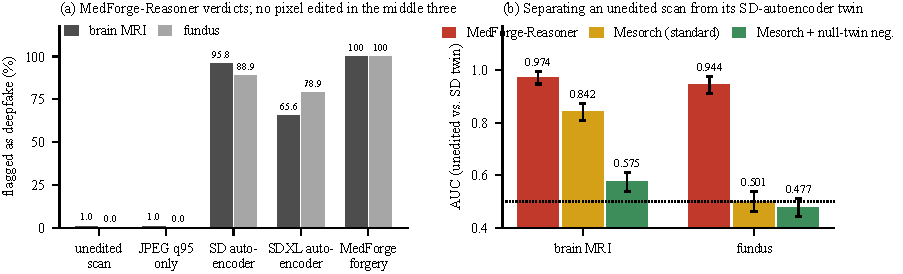
\includegraphics[width=0.98\linewidth]{figures/fig_medforge.pdf}
\caption{\textbf{MedForge's own detector responds to the autoencoder.} (a) MedForge-Reasoner's ``deepfake'' verdicts per modality on 96 brain-MRI and 90 fundus untouched MedForge test scans, % src: docs/council/round3/experiments/local/r3_box_audit.csv (n per arm)
the same scans after JPEG re-encoding or an autoencoder round trip with no edit, and 48 MedForge forgeries. % src: paper/data/medforge_reasoner_hardlabel.csv
(b) AUC separating an untouched scan from its SD-autoencoder twin, with 95\% intervals. Standard Mesorch responds to the twin on brain MRI, which it was trained on, but not on fundus, which it has never seen. Values await confirmation on a fresh sample (\TODO{E3b: fresh sample}).}
\label{fig:medforge}
\end{figure*}

\paragraph{MedForge.}
To test whether the response is an artefact of our own pipeline, we sampled untouched scans from MedForge-90K's test split (brain MRI and fundus) and built three versions that edit nothing: a JPEG re-save at quality 95, which is how MedForge stores its forgeries, % src: docs/council/round2/experiments/README.md (harness fact 6); E2_medforge_confound.md (JPEG step)
and SD- and SDXL-autoencoder round trips followed by the same JPEG step.
MedForge-Reasoner~\cite{chen2026medforge}, an 8B vision-language detector, % src: docs/council/round2/landscape_and_odds.md (Sec. 1)
flags all 48 forgeries we sampled and 1 of 186 untouched scans (\cref{tab:medforge,fig:medforge}). % src: paper/data/medforge_reasoner_hardlabel.csv
After an SD-autoencoder round trip it flags 95.8\% of brain MRI and 88.9\% of fundus scans, % src: docs/council/round3/experiments/local/r3_box_audit.csv (N_sd, real)
and after an SDXL round trip 65.6\% and 78.9\%. % src: docs/council/round3/experiments/local/r3_box_audit.csv (N_sdxl, real)
Its fingerprint share is 0.92 for the SD round trip and 0.72 for SDXL. % src: paper/data/medforge_fingerprint_share.json (derived from work/e0/out_local/e2/e2_table.csv)
The verdicts are localised.
Every one of its 306 ``deepfake'' calls on an unedited round trip comes with a box, and no ``real'' call does; % src: docs/council/round3/experiments/local/R3_STEP1_REPORT.md (Sec. 1)
the median box covers 2.0\% of a brain scan and 3.9\% of a fundus image, % src: docs/council/round3/experiments/local/r3_box_audit.csv (N_sd, real, area_median)
against 3.6\% and 2.3\% for its boxes on real MedForge forgeries. % src: docs/council/round3/experiments/local/r3_box_audit.csv (R, forged, area_median)
On 22 of the 30 sampled scans labelled normal (12 of 16 brains), it reports a localised manipulation after the SD round trip, % src: docs/council/round3/experiments/local/r3_box_audit_normals.csv (N_sd)
and for the same source its SD and SDXL boxes overlap with a median IoU of 0.83 (133 sources; 0.056 for shuffled sources), % src: docs/council/round3/experiments/local/R3_STEP1_REPORT.md (Sec. 1); r3_chairman_crosscheck.csv
so the box follows the image content rather than a fixed prior location: the Reasoner describes a lesion-sized edit that does not exist.
The JPEG version scores 0.500, % src: work/e0/out_local/e2/e2_table.csv
but it is a far milder change (57.5--64.6\,dB PSNR to the untouched scan, against 38.1--39.5\,dB for the SD round trip), % src: docs/council/round3/experiments/local/r3_chairman_crosscheck.csv (per-modality medians)
so it does not show that non-neural processing of the same strength would pass. \TODO{E3b: JPEG, JPEG 2000 and a learned codec at the SD round trip's PSNR; local SD null; fresh sample}
Standard Mesorch, trained only on our data, shows the same response on MedForge brain MRI (0.842) % src: work/e0/out_local/e2/e2_table.csv
and none on fundus (0.501), a modality it has never seen; % src: work/e0/out_local/e2/e2_table.csv
twin negatives cut it to 0.575, % src: work/e0/out_local/e2/e2_table.csv
although neither Mesorch variant detects MedForge's own forgeries (0.521 and 0.555). % src: work/e0/out_local/e2/e2_table.csv

\paragraph{A held-out generator, and twin training.}
The same response appears with SDXL, which no model saw in training: standard Mesorch separates untouched sources from their SDXL twins at 0.842, % src: docs/council/round2/experiments/README.md (Step 5)
twin-trained Mesorch at 0.601. % src: docs/council/round2/experiments/README.md (Step 5)
Training Mesorch with twins as negatives lifts B-vs-C from 0.536 to 0.743, % src: work/e0/out_local/tables/table_main.csv
and distillation from the paired model to 0.768. % src: work/e0/out_local/tables/e9_final_comparison.csv
The gain is specific to the backbone: of five backbones trained the same way, only Mesorch gains more than 0.10 (MVSS-Net $+$0.023, TruFor $-$0.010). % src: work/e0/out_local/tables/E2_REPORT.md (Step 1)
It does not reach CT, which stays at 0.567, % src: work/e0/out_local/tables/table_main.csv
and it leaves a residual false alarm, A-vs-B 0.704 (\cref{sec:shortcuts}). % src: work/e0/out_local/tables/table_main.csv

\subsection{Operating points: no detector wins everywhere}
\label{sec:operating}

\begin{table*}[t]
\centering
\caption{\textbf{Operating points.} One threshold per detector, fixed at 95\% TPR on calibration SD injections pooled over modalities; every rate is read at that threshold. Cells give pooled\,/\,CT, in \%. Rates are on calibration except ``SD twin, test''; rows marked $^{\ddagger}$ are on test throughout, because their calibration scores are not stored locally. $^{\circ}$Held out of training for the last three rows; no other row saw any benign operation. ``SDXL twin'': FPR on calibration SDXL twins\,/\,on SD twins matched to them on in-mask MSE ($\star$: pending, \TODO{E3a: SDXL holdout and MSE-matched SD nulls}); not computed for CT. ``worst'': maximum FPR over the calibration SD twins (test for $^{\ddagger}$ rows), untouched sources and the four benign operations. AE: autoencoder round trip of the whole source. Per-modality rows are in the supplementary material.}
\label{tab:op}
\footnotesize
\setlength{\tabcolsep}{2.3pt}
\begin{tabular}{@{}lcccccccccc@{}}
\toprule
 & & \multicolumn{2}{c}{SD twin} & & \multicolumn{4}{c}{benign operation on the source} & & \\
\cmidrule(lr){3-4}\cmidrule(lr){6-9}
Detector & TPR & cal. & test & untouched & JPEG & VQ-AE & NL-means$^{\circ}$ & SDXL-AE$^{\circ}$ & SDXL twin & worst \\
\midrule
\multicolumn{11}{@{}l}{\emph{Single image (Mesorch)}}\\
standard & 94.9\,/\,72.6 & 93.3\,/\,68.4 & 95.2\,/\,78.5 & 35.0\,/\,63.2 & 32.8\,/\,63.2 & 53.6\,/\,71.4 & 64.4\,/\,74.6 & 47.9\,/\,65.4 & 82.9\,/\,$\star$ & 93.3\,/\,74.6 \\ % src: docs/council/round3/experiments/local/r3_operating_points.csv (V0, ALL / ct); SDXL twin: R3_STEP1_REPORT.md Sec. 4 (E0e, carried over)
+ null twins & 94.9\,/\,72.6 & 94.0\,/\,70.5 & 95.6\,/\,73.6 & 84.1\,/\,66.5 & 89.2\,/\,84.9 & 87.5\,/\,69.7 & 94.9\,/\,87.6 & 84.1\,/\,68.6 & 90.9\,/\,$\star$ & 94.9\,/\,87.6 \\ % src: docs/council/round3/experiments/local/r3_operating_points.csv (V1, ALL / ct); SDXL twin: R3_STEP1_REPORT.md Sec. 4 (E0e)
+ distilled$^{\ddagger}$ & 95.9\,/\,91.7 & -- & 72.3\,/\,89.3 & 41.2\,/\,87.4 & 38.1\,/\,73.6 & 48.0\,/\,87.0 & 54.0\,/\,82.1 & 40.2\,/\,83.3 & 61.3\,/\,$\star$ & 72.3\,/\,89.3 \\ % src: docs/council/round3/experiments/local/r3_operating_points.csv (V1d, ALL / ct, test, tpr_test_C_sd); SDXL twin: R3_STEP1_REPORT.md Sec. 4 (E0e)
\midrule
\multicolumn{11}{@{}l}{\emph{Null-twin reference}}\\
subtraction & 94.9\,/\,91.6 & 43.8\,/\,14.7 & 46.7\,/\,12.4 & 12.0\,/\,2.7 & 15.3\,/\,4.3 & 99.3\,/\,100 & 26.3\,/\,41.1 & 98.4\,/\,100 & $\star$ & 99.3\,/\,100 \\ % src: docs/council/round3/experiments/local/r3_operating_points.csv (sub_raw, ALL / ct)
\quad standardised & 94.9\,/\,91.6 & 14.9\,/\,14.7 & 12.1\,/\,11.6 & 1.0\,/\,2.7 & 4.1\,/\,4.3 & 72.5\,/\,100 & 21.0\,/\,38.9 & 83.9\,/\,100 & $\star$ & 83.9\,/\,100 \\ % src: docs/council/round3/experiments/local/r3_operating_points.csv (sub_std, ALL / ct)
paired (FC-Siam-diff)$^{\ddagger}$ & 97.0\,/\,86.0 & -- & 13.6\,/\,5.8 & 1.7\,/\,0.0 & 19.6\,/\,41.1 & 38.4\,/\,91.5 & 78.4\,/\,98.8 & 70.6\,/\,96.7 & 5.5\,/\,$\star$ & 78.4\,/\,98.8 \\ % src: docs/council/round3/experiments/local/r3_operating_points.csv (p1n, ALL / ct, test, tpr_test_C_sd); SDXL twin: R3_STEP1_REPORT.md Sec. 4 (E0e)
+ benign negatives & 94.9\,/\,77.9 & 11.1\,/\,4.2 & 10.1\,/\,1.7 & 0.2\,/\,0.0 & 0.5\,/\,0.0 & 10.1\,/\,25.4 & 11.8\,/\,8.1 & 26.9\,/\,52.4 & $\star$ & 26.9\,/\,52.4 \\ % src: docs/council/round3/experiments/local/r3_operating_points.csv (p2, ALL / ct)
\quad + invariance, $\lambda$=0.03 & 94.9\,/\,80.0 & 6.0\,/\,7.4 & 6.1\,/\,3.3 & 0.1\,/\,0.0 & 0.0\,/\,0.0 & 4.3\,/\,9.7 & 1.5\,/\,0.0 & 8.8\,/\,20.5 & $\star$ & \textbf{8.8}\,/\,\textbf{20.5} \\ % src: docs/council/round3/experiments/local/r3_operating_points.csv (p3_0.03, ALL / ct)
\quad + invariance, $\lambda$=0.1 & 94.9\,/\,78.9 & 27.8\,/\,60.0 & 29.0\,/\,62.0 & 18.2\,/\,8.6 & 8.8\,/\,0.5 & 24.2\,/\,33.0 & 12.9\,/\,10.3 & 26.3\,/\,32.4 & $\star$ & 27.8\,/\,60.0 \\ % src: docs/council/round3/experiments/local/r3_operating_points.csv (p3_0.1, ALL / ct)
\bottomrule
\end{tabular}
\end{table*}

\begin{figure}[t]
\centering
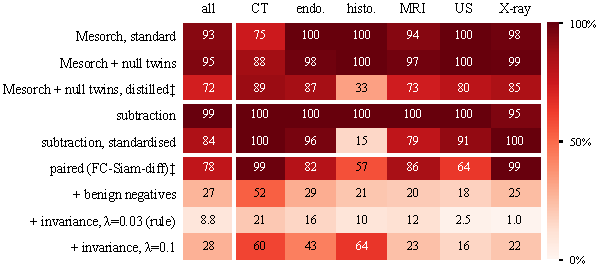
\includegraphics[width=\linewidth]{figures/fig_operating.pdf}
\caption{\textbf{Worst false-positive rate per modality} (\%), over SD twins, untouched sources and four benign operations, at each detector's pooled calibration threshold (95\% TPR on SD injections). Rows as in \cref{tab:op}; $^{\ddagger}$test-split rates. No row is light in every column.}
\label{fig:operating}
\end{figure}

\Cref{tab:op,fig:operating} put every Mesorch-based and reference-based detector at one threshold and read it against each negative type.
No detector wins everywhere, and a high AUC does not imply a usable operating point.
Fine-tuned single-image detectors flag 93.3\% (standard) and 94.0\% (twin-trained) of calibration SD twins, % src: docs/council/round3/experiments/local/r3_operating_points.csv (V0, V1, fpr_cal_SD_null)
so their AUC margins carry no alarm rate a user could live with.
Subtraction, at AUC 0.921, flags 43.8\% of calibration and 46.7\% of test SD twins, % src: docs/council/round3/experiments/local/r3_operating_points.csv (sub_raw, fpr_cal_SD_null, fpr_test_SD_null)
and 99.3\% and 98.4\% of sources round-tripped through the VQ and SDXL autoencoders. % src: docs/council/round3/experiments/local/r3_operating_points.csv (sub_raw, fpr_vqvae, fpr_sdxlvae)
Standardising it per modality lifts its AUC to 0.976 % src: docs/council/round3/experiments/local/r3_subtraction_standardised.csv (standardised, ALL)
but still flags 72.5\% and 83.9\% of those round trips, % src: docs/council/round3/experiments/local/r3_operating_points.csv (sub_std, fpr_vqvae, fpr_sdxlvae)
and all of them on CT.
The paired baseline flags 13.6\% of test SD twins, % src: docs/council/round3/experiments/local/r3_operating_points.csv (p1n, fpr_test_SD_null)
but 78.4\% of denoised and 70.6\% of SDXL-autoencoded sources (98.8\% and 96.7\% on CT). % src: docs/council/round3/experiments/local/r3_operating_points.csv (p1n, fpr_nlmeans, fpr_sdxlvae, ALL / ct)
On CT every detector is weaker at the pooled threshold; single-image Mesorch recalls 72.6\% of injections. % src: docs/council/round3/experiments/local/r3_operating_points.csv (V0, V1, ct, tpr_cal_C_sd)

\paragraph{Drift beside transfer.}
Thresholds drift even without a change of generator: the twin-trained model's SD-twin FPR moves from 94.0\% on calibration to 95.6\% on test, and subtraction's from 43.8\% to 46.7\%. % src: docs/council/round3/experiments/local/r3_operating_points.csv (V1, sub_raw: fpr_cal_SD_null, fpr_test_SD_null)
A raw cross-generator rate is not comparable with these: the paired baseline flags 5.5\% of SDXL twins, less than the 13.6\% it flags on SD twins, % src: docs/council/round3/experiments/local/R3_STEP1_REPORT.md (Sec. 4, E0e carried over); r3_operating_points.csv (p1n, fpr_test_SD_null)
because an SDXL twin sits about 7$\times$ closer to its source (in-mask MSE 1.83 against 13.54) and is an easier negative. % src: docs/council/round2/experiments/README.md (Step 5)
Transfer is therefore read against SD twins matched on in-mask MSE (\TODO{E3a: MSE-matched SD-null FPR}).

\paragraph{AUC and operating-point selection disagree.}
For the paired baseline with an invariance penalty, choosing $\lambda$ by how little the output changes under benign processing picks $\lambda=0.1$; % src: round3/council_verdict.md (pending r3_step1) (Where the Council Clashes: lambda=0.1 was chosen by AUC deviation)
at its threshold that model flags 18.2\% of untouched calibration sources (20.2\% on test) and 27.8\% of SD twins. % src: docs/council/round3/experiments/local/r3_operating_points.csv (p3_0.1: fpr_A, fpr_A_test, fpr_cal_SD_null)
Our pre-registered rule (\cref{sec:protocol}) picks $\lambda=0.03$ instead, whose worst calibration FPR over the five selection negatives is 6.0\%, against 11.8\% without the penalty and 27.8\% and 43.3\% for $\lambda=0.1$ and 0.3. % src: docs/council/round3/experiments/local/r3_lambda_preregistration.json (max_fpr)

\subsection{Reference-verification baselines}
\label{sec:refverif}

\begin{table}[t]
\centering
\caption{\textbf{Reference-verification baselines} (test AUC). All use the null-twin reference. ``worst FPR'': pooled\,/\,CT, in \%, from \cref{tab:op}. $^{\P}$Post-selection on test (see text). $^{\ddagger}$Test-split rates.}
\label{tab:refverif}
\footnotesize
\setlength{\tabcolsep}{3pt}
\begin{tabular}{@{}lcccc@{}}
\toprule
Baseline & B-vs-C & CT & B-vs-D & worst FPR \\
\midrule
subtraction, 0 parameters & 0.921 & \textbf{0.960} & \textbf{0.999} & 99.3\,/\,100 \\ % src: work/e0/out_local/e0x/e0a/E0A_REPORT.md; worst FPR: docs/council/round3/experiments/local/r3_operating_points.csv (sub_raw)
\quad standardised & 0.976 & \textbf{0.960} & -- & 83.9\,/\,100 \\ % src: docs/council/round3/experiments/local/r3_subtraction_standardised.csv; r3_operating_points.csv (sub_std)
block-wise robust hash & \multicolumn{4}{c}{\PENDING{E3c}} \\
paired (FC-Siam-diff)$^{\P}$ & \textbf{0.984} & 0.927 & 0.996 & 78.4\,/\,98.8$^{\ddagger}$ \\ % src: paper/data/paired_family_test_auc.csv (derived); r3_operating_points.csv (p1n)
\quad + benign negatives$^{\P}$ & 0.978 & 0.952 & 0.994 & 26.9\,/\,52.4 \\ % src: paper/data/paired_family_test_auc.csv (derived, p2); docs/council/round3/experiments/local/r3_operating_points.csv (p2)
\quad\quad + invariance, $\lambda$=0.03$^{\P}$ & 0.982 & 0.934 & 0.997 & \textbf{8.8}\,/\,\textbf{20.5} \\ % src: paper/data/paired_family_test_auc.csv (derived, p3 lam=0.03); docs/council/round3/experiments/local/r3_operating_points.csv (p3_0.03)
\bottomrule
\end{tabular}
\end{table}

When a reference image is available, detection becomes verification against it (\cref{tab:refverif}).
Every row here uses the null-twin reference, not a pristine original; rescoring with the source as reference is pending (\TODO{E3a: pristine-reference rescoring}).
A zero-parameter subtraction reaches 0.921 [0.910, 0.931] on B-vs-C, % src: docs/council/round3/experiments/local/r3_subtraction_standardised.csv (raw, ALL)
and 0.976 [0.968, 0.982] once its score is standardised per modality on calibration twins. % src: docs/council/round3/experiments/local/r3_subtraction_standardised.csv (standardised, ALL)
Telling it the true mask adds nothing (0.9208 against 0.9210), % src: work/e0/out_local/e0x/e0a/E0A_REPORT.md
whereas a byte-level hash is at chance (0.506), % src: work/e0/out_local/e0x/e0a/E0A_REPORT.md
because every image differs from the reference across the whole feather.
The paired model's control, trained on identical rows without the reference, scores 0.726, % src: work/e0/out_local/tables/e3_table_bar.csv (pairnet_single)
so the reference is what makes the task easy, and any claim that \dataset is hard must read ``hard without a reference''.

The paired baseline, FC-Siam-diff on a Mesorch trunk with the LaMa null twin as reference, reaches 0.984. % src: work/e0/out_local/tables/e3_table_bar.csv
This number is post-selection: variants of this paired model family were revised after their test scores had been read, so it is optimistic. % src: docs/council/round3/council_verdict.md (Blind Spots: the test split is spent for PAIR-NET-family claims)
Its margin over raw subtraction, $+$0.063 [0.053, 0.073], % src: docs/council/round3/experiments/local/r3_subtraction_gap_to_p1n.csv (raw, ALL)
shrinks to $+$0.008 [0.001, 0.016] over standardised subtraction, % src: docs/council/round3/experiments/local/r3_subtraction_gap_to_p1n.csv (standardised, ALL)
so almost all of it is per-modality calibration.
Per modality, the paired baseline still leads on endoscopy ($+$0.074) and trails on CT ($-$0.033). % src: docs/council/round3/experiments/local/r3_subtraction_gap_to_p1n.csv (standardised, endoscopy, ct)
At its operating point it does not separate an edit from benign reprocessing either (\cref{tab:op}).

Adding JPEG and VQ-autoencoder copies of sources as negatives, and then an output-invariance penalty, changes the operating point far more than the AUC.
Of the detectors tested, only a reference-paired verifier trained with benign negatives and an output-invariance penalty keeps FPR under 10\% on every negative type at one threshold; we report it as a baseline. % src: docs/council/round3/experiments/local/r3_operating_points.csv (p3_0.03, ALL, worst_fpr 0.088)
\PENDING{Pending E3a (pristine-reference rescoring and SDXL holdout).}
The statement is pooled over modalities, where its worst rate is 8.8\%, on the held-out SDXL autoencoder; % src: docs/council/round3/experiments/local/r3_operating_points.csv (p3_0.03, ALL, worst_fpr_on fpr_sdxlvae)
its SD-twin rate barely drifts (6.0\% on calibration, 6.1\% on test). % src: docs/council/round3/experiments/local/r3_operating_points.csv (p3_0.03, fpr_cal_SD_null, fpr_test_SD_null)
$\lambda=0.03$ was set by the min--max calibration FPR rule, written down before any SDXL score was read; the rule is not blind, since its calibration inputs had been inspected, but it locks the choice before the held-out generator and further seeds are scored. % src: docs/council/round3/experiments/local/r3_lambda_preregistration.json (honesty_note)
Its B-vs-C AUC of 0.982 is within 0.01 of standardised subtraction, so we make no AUC claim for it. % src: paper/data/paired_family_test_auc.csv (derived, p3 lam=0.03, b_vs_c)
On CT it is weak: it flags 20.5\% of SDXL-autoencoded scans and recalls 80.0\% of injections at the pooled threshold, % src: docs/council/round3/experiments/local/r3_operating_points.csv (p3_0.03, ct: fpr_sdxlvae, tpr_cal_C_sd)
and it rests on one seed (\TODO{E3d: seeds 43 and 44}).
Like the paired baseline's, its test AUC is post-selection, since the family's test scores had been read.

\subsection{Finding the edit versus judging it}
\label{sec:oracle}

\begin{table}[t]
\centering
\caption{\textbf{Oracle mask} (single image, Mesorch + null twins, calibration only; these models' test tables are sealed). Mean of three seeds where marked, SD $\leq$ 0.015. % src: paper/data/oracle_calibration_3seed.csv (std column)
}
\label{tab:oracle}
\footnotesize
\setlength{\tabcolsep}{3pt}
\begin{tabular}{@{}lccccc@{}}
\toprule
 & B-vs-C & CT & B-vs-D & CT B-vs-D & A-vs-B (0.5) \\
\midrule
3 seeds & 0.724 & 0.546 & 0.786 & 0.538 & 0.708 \\ % src: paper/data/oracle_calibration_3seed.csv (derived; matches README Step 8)
\quad read inside true mask & 0.723 & 0.534 & 0.737 & 0.480 & 0.858 \\ % src: work/e0/out_local/e0x/e0b/open/e0b_calibration.csv (e0b_v1pool, score_max_in)
zero-mask channel & 0.726 & 0.540 & 0.784 & 0.536 & 0.710 \\ % src: work/e0/out_local/e0x/e0b/open/e0b_calibration.csv (e0b_zeros_s42)
true-mask channel, 3 seeds & \textbf{0.794} & 0.534 & \textbf{0.936} & \textbf{0.828} & 0.683 \\ % src: paper/data/oracle_calibration_3seed.csv (derived; matches README single results sheet, step 4)
\bottomrule
\end{tabular}
\end{table}

As a diagnostic, we ask why single-image detection stays hard: either the detector cannot \emph{find} a 0.1\%-of-frame edit, % src: docs/council/context_dossier.md (A, mask areas: CT 0.11-0.14%)
or it finds the region but cannot \emph{judge} whether it was edited.
We retrain twin-trained Mesorch with the true mask as a fourth input channel, given to every image of a lineage so it carries no label, beside a control whose channel is all zeros (\cref{tab:oracle}; per modality in the supplementary material).
The control reproduces the original model within 0.0033, % src: work/e0/out_local/e0x/e0b/open/e0b_verdict.json
and zeroing the channel at inference costs the oracle 0.25, so the channel is used. % src: work/e0/out_local/e0x/e0b/open/e0b_verdict.json
The mask raises injection from 0.724 to 0.794 % src: paper/data/oracle_calibration_3seed.csv (derived)
and removal from 0.786 to 0.936. % src: paper/data/oracle_calibration_3seed.csv (derived)
Removal is a finding problem only on CT, where the mask is worth $+$0.29 (0.538 to 0.828); % src: paper/data/oracle_calibration_3seed.csv (derived)
outside CT, removal is already at 0.93--0.99 without it. % src: paper/data/oracle_calibration_3seed.csv (derived)
CT injection does not move (0.546 to 0.534): told where the lesion is, the model still cannot tell it from the twin, so it is a judging problem. % src: paper/data/oracle_calibration_3seed.csv (derived)
Reading the frozen model's map only inside the true mask helps nowhere (injection 0.724 to 0.723, removal 0.786 to 0.737). % src: paper/data/oracle_calibration_3seed.csv (derived)
Nor does reading the sampler directly: a training-free probe of the frozen SD inpainting UNet's noise-prediction error inside the mask is at chance (0.508, against 0.507 for its autoencoder-only control; supplementary). % src: work/e0/out_local/e1_irp/E1_REPORT.md; e1_criteria.json

\subsection{Shortcuts}
\label{sec:shortcuts}

Twin-trained Mesorch raises its score on the twin of an injection lineage far more than on that of a removal lineage ($+$0.283 against $+$0.067 over the source, calibration). % src: docs/council/round2/experiments/README.md (Step 1); docs/council/round2/experiments/local/e0c_calibration_verdict.json
Compositing each rebuilt twin through the other family's rescaled mask, so that only the outline changes, moves the score by $-$0.005 [$-$0.020, 0.010] for injection and $+$0.026 [0.008, 0.045] for removal, % src: docs/council/round2/experiments/README.md (Step 2a); work/e0/out_local/e0x/e0c3/e0c3_table.csv
an order of magnitude below the $\pm$0.12 that a shape explanation required. % src: docs/council/round2/experiments/README.md (Step 2a)
The false alarm sits where the autoencoder worked: read only inside the mask, A-vs-B rises to 0.858, % src: work/e0/out_local/e0x/e0b/open/e0b_calibration.csv (e0b_v1pool, score_max_in)
and only outside it, 0.423. % src: work/e0/out_local/e0x/e0b/open/e0b_calibration.csv (e0b_v1pool, score_max_out)
Mask geometry remains a shortcut for anything that compares families (up to 0.950, \cref{sec:family}). % src: work/e0/out_local/e0x/e0d/e0d_shape.csv

\subsection{Localisation}
\label{sec:loc}

\begin{table}[t]
\centering
\caption{\textbf{Localisation} (test, per-image pixel F1). ``np'': null-penalised (\cref{eq:np}). $t^\ast$ is chosen on calibration. Reference-based models are void here, since the reference reveals where the edit is.}
\label{tab:loc}
\footnotesize
\setlength{\tabcolsep}{4pt}
\begin{tabular}{@{}llcccc@{}}
\toprule
 & Mesorch ($t^\ast$) & F1@0.5 & np@0.5 & F1@$t^\ast$ & np@$t^\ast$ \\
\midrule
\multirow{3}{*}{\rotatebox{90}{inject.}} & standard (0.35) & \textbf{0.779} & 0.536 & \textbf{0.782} & 0.533 \\ % src: work/e0/out_local/e0x/e0d/e0d_partb.csv (rule, tstar, null_penalised rows); e0d_tstar.json
 & + null twins (0.10) & 0.557 & 0.501 & 0.699 & 0.531 \\ % src: work/e0/out_local/e0x/e0d/e0d_partb.csv; e0d_tstar.json
 & + distilled (0.15) & 0.565 & 0.501 & 0.710 & \textbf{0.548} \\ % src: work/e0/out_local/e0x/e0d/e0d_partb.csv; e0d_tstar.json
\midrule
\multirow{3}{*}{\rotatebox{90}{remove}} & standard (0.35) & \textbf{0.594} & 0.414 & 0.598 & 0.414 \\ % src: work/e0/out_local/e0x/e0d/e0d_partb.csv
 & + null twins (0.10) & 0.514 & 0.506 & 0.575 & 0.533 \\ % src: work/e0/out_local/e0x/e0d/e0d_partb.csv
 & + distilled (0.15) & 0.525 & \textbf{0.518} & \textbf{0.605} & \textbf{0.553} \\ % src: work/e0/out_local/e0x/e0d/e0d_partb.csv
\bottomrule
\end{tabular}
\end{table}

Read in the usual way, standard Mesorch localises best (\cref{tab:loc}): injection F1 0.779 against 0.557 for the twin-trained model. % src: work/e0/out_local/e0x/e0d/e0d_partb.csv
Most of that lead is marking every region the autoencoder touched: standard Mesorch predicts forged pixels on 82\% of null twins, the twin-trained model on 37\%. % src: docs/council/round2/experiments/local/e0d_null_penalised.csv (null_any_fp)
Charging those pixels shrinks the lead to 0.536 against 0.501, % src: work/e0/out_local/e0x/e0d/e0d_partb.csv (null_penalised, t=0.5)
and at calibration-chosen thresholds the two are indistinguishable (0.533 against 0.531). % src: work/e0/out_local/e0x/e0d/e0d_partb.csv (null_penalised at t*)
The threshold matters more than the model: moving the twin-trained model from 0.5 to its calibrated 0.10 is worth $+$0.142. % src: work/e0/out_local/e0x/e0d/E0D_PARTB.md; docs/council/round2/experiments/README.md (Step 6)
CT injection localisation is 0.049 at 0.5. % src: docs/council/round2/experiments/local/e0d_null_penalised.csv (V1, C_sd, ct, f1_pos_only)

\section{Limitations}
\label{sec:limitations}

\textbf{Healthy sources.} Only CT injections are placed in tissue verified healthy by four readers; the other modalities' injection sources carry image-level labels at best, so an injected lesion may sit beside unannotated pathology.
\textbf{Image format.} All images are 8-bit 2D renders: there are no Hounsfield units, k-space or volumes, and split units hold 1.01--1.36 lineages, % src: docs/council/context_dossier.md (A, No 3D)
so inter-slice consistency cannot be exploited.
\textbf{Mask-shape shortcut.} Removal masks are traced lesions and injection masks are synthetic, and geometry alone separates the families (up to 0.950 held out); % src: work/e0/out_local/e0x/e0d/e0d_shape.csv
we report families separately but do not remove the cue.
\textbf{Removal quality.} Removal is attempted, not guaranteed; per-lineage efficacy is published, and outside CT the contours come from a single annotator.
\textbf{Generators.} Two generators are used for training and one is held out; the twin matches the autoencoder, not the sampler.
\textbf{MedForge study.} It covers brain MRI and fundus on 186 untouched scans for the Reasoner; % src: paper/data/medforge_reasoner_hardlabel.csv
chest X-ray is not evaluated because its sources require credentialed access, and 8.3\% of the sampled brain-MRI scans duplicate our MRI sources. % src: docs/council/round2/experiments/README.md (Step 9, job A)
\textbf{MedForge degradation control.} The JPEG version is a much milder change than the autoencoder round trip, so we cannot yet say whether non-neural processing of the same strength would also be called fake (\TODO{E3b}).
\textbf{Reference.} Every reference-based row compares against the LaMa null twin, not a pristine original, and assumes pixel registration.
\textbf{Test reuse.} The paired model family was revised after its test scores had been read, so its test AUCs are post-selection; its $\lambda$ rule is calibration-only but not blind, and the invariance baseline rests on one seed (\TODO{E3d}).
\textbf{No reader study.} We have not measured whether radiologists can see these edits or whether an edit changes a diagnosis.
\textbf{CT.} Single-image CT detection remains near chance (best 0.586), % src: paper/data/main_benchmark_test.csv (derived)
and no detector we test reaches a 10\% worst-case FPR on CT at the pooled threshold. % src: docs/council/round3/experiments/local/r3_operating_points.csv (worst_fpr, ct: minimum 0.205)

\section*{Ethics statement}
\textbf{Dual use.} A forgery corpus could help train better forgers. Every edit is produced by public, off-the-shelf generators, so \dataset adds no attack capability that is not already available; what it adds is the null twin, which serves only measurement and defence.
\textbf{Licences.} Sources are public, de-identified research datasets. Each derived image is released under terms compatible with its source, listed per source in the supplementary licence table; sources whose redistribution terms are unclear are released as generation scripts and manifests rather than images. \TODO{complete the licence table; resolve the repackaged Kaggle sources}
MedForge-90K is used under its C-UDA licence: no MedForge image, and no image derived from one, is shown or released.
\textbf{Privacy.} CT headers are reduced to a whitelist of non-identifying fields with salted identifiers, and no DICOM header ships. No new human-subject data was collected.
\textbf{Release.} Access is gated behind a research-use agreement that forbids clinical deception and re-identification, with a datasheet~\cite{gebru2021datasheets} describing composition, intended uses and known shortcuts.

\section{Conclusion}
A medical forgery detector that is scored against untouched images is largely scored on whether it recognises the generator's autoencoder, and MedForge's own detector draws lesion-sized boxes on images nobody edited.
\dataset makes that visible by giving every edit a twin that went through the same autoencoder unedited, and its protocol reads one calibration operating point against every kind of unedited image, per modality.
Measured this way, single-image detection is far from solved, reference-based AUC is mostly per-modality arithmetic, and no detector we test has an acceptable false-alarm rate on every negative type and modality.
The open problems are concrete: judging small CT injections, finding CT removals, and a verifier whose operating point survives benign neural processing on CT.

{
    \small
    \bibliographystyle{ieeenat_fullname}
    \bibliography{refs}
}

% Supplementary material (outline): uncomment to compile it after the paper, then split the
% pages off before submitting, as the author kit recommends.
% % Supplementary material: OUTLINE ONLY.
% Following the author kit, compile it after the main paper by uncommenting
% % Supplementary material: OUTLINE ONLY.
% Following the author kit, compile it after the main paper by uncommenting
% % Supplementary material: OUTLINE ONLY.
% Following the author kit, compile it after the main paper by uncommenting
% \input{sec/X_suppl} in main.tex, then split the pages off before submitting.
% Supplementary deadline (AoE): Nov 23, 2026 (docs/council/round2/landscape_and_odds.md, Sec. 3).

\clearpage
\setcounter{page}{1}
\maketitlesupplementary

\section{Datasheet}
\label{sec:supp:datasheet}
\TODO{Write following Gebru \etal~\cite{gebru2021datasheets}.}
\begin{itemize}[leftmargin=*,itemsep=1pt]
\item \textbf{Motivation:} measuring how much of a forgery detector's score is the generator's autoencoder.
\item \textbf{Composition:} lineages by modality $\times$ edit family $\times$ split (training / calibration / test), with image counts per variant; mask-area distributions; removal efficacy per lineage; near-duplicate flags; SDXL images (calibration and test only).
\item \textbf{Collection and preprocessing:} CT rendering window and header whitelist; source linking and de-duplication across annotated corpora and their repackages; mask processing; generation settings; compositing rule; release audits.
\item \textbf{Uses:} intended (forensic evaluation, robustness research); out of scope (clinical use, training forgers, re-identification). Known shortcuts: mask geometry separates families; removal is attempted, not guaranteed.
\item \textbf{Distribution and maintenance:} gated access, research-use agreement, versioning, contact (anonymised for review).
\end{itemize}

\section{Licence table}
\label{sec:supp:licence}
\TODO{One row per source: dataset, original licence, whether redistribution of derived images is permitted, what we release (images, or generation scripts and manifests only), required attribution. Open items: the repackaged Kaggle sources for X-ray, histopathology, MRI and non-removal endoscopy and ultrasound have no recorded upstream licence.}
\begin{itemize}[leftmargin=*,itemsep=1pt]
\item LIDC-IDRI~\cite{armato2011lidc}; HyperKvasir~\cite{borgli2020hyperkvasir}; Kvasir-SEG~\cite{jha2020kvasirseg}; LC25000~\cite{borkowski2019lc25000}; brain-tumour MRI aggregate~\cite{nickparvar2021brainmri}; Cheng \etal\ masks~\cite{cheng2015brain}; BUSI~\cite{aldhabyani2020busi}; TB radiographs~\cite{rahman2020tb}.
\item Generators: SD-1.5 inpainting, big-LaMa, SDXL inpainting 0.1 and its fp16-fix autoencoder (model licences and pinned revisions).
\item MedForge-90K (C-UDA): used for evaluation only; nothing derived from it is released.
\end{itemize}

\section{Generation details}
\begin{itemize}[leftmargin=*,itemsep=1pt]
\item Pinned model revisions, scheduler, steps, guidance, strength and resolution per generator; per-modality prompts and negative prompts.
\item Crop and resize path; null-twin construction; compositing (feathered alpha, rounding, exact pass-through where the mask is zero); grayscale handling.
\item Quality checks: outside-mask bit identity, degenerate twins, in-mask twin fidelity (SD against SDXL), contact sheets.
\end{itemize}

\section{Full per-modality results}
\begin{itemize}[leftmargin=*,itemsep=1pt]
\item \Cref{tab:main} per modality, for every detector and task (source: \texttt{paper/data/main\_benchmark\_test.csv}).
\item Localisation per modality and edit family, raw and null-penalised, at 0.5 and $t^\ast$, with the mask-shape baseline beside each family.
\item Operating points (\cref{tab:op}) for every modality, every detector including $\lambda=0.3$, and the removal-lineage SD twins and LaMa twins as further negative types (source: \texttt{paper/data/operating\_points.csv}).
\item Held-out SDXL per modality, including removal, with the MSE-matched SD-twin comparison. \TODO{E3a}
\item Oracle-mask study per modality and seed (calibration only).
\item MedForge per modality and per twin (brain MRI, fundus), with the duplicate-exclusion details.
\end{itemize}

\section{Additional analyses}
\begin{itemize}[leftmargin=*,itemsep=1pt]
\item Leave-one-modality-out and leave-one-generator-out training; training-set size (25\%, 50\%, 100\%). % src: work/e0/out_local/tables/table_main.csv (nai_v1/frac25, frac50)
\item The paired-operator variants that tied or lost against absolute difference, and distillation.
\item Benign-processing suite in full (both directions, per operation, with per-arm score spreads), the output-level invariance penalty, and the pre-registered $\lambda$ rule with its input hashes.
\item Invariance-baseline seeds 43 and 44 (mean $\pm$ SD; any seed whose worst pooled FPR exceeds 0.20 is reported on its own). \TODO{E3d}
\item Block-wise robust hash at 16 and 32 px. \TODO{E3c}
\item Mask-swap test and in-mask versus out-of-mask false alarms.
\item MedForge box audit in full: box-area distributions per arm, the 30 normal scans, and SD-versus-SDXL box overlap against a shuffled-source baseline.
\item Classical copy-move detection (SIFT and RANSAC) as a generator-free baseline on A-vs-CM.
\end{itemize}

\paragraph{A falsified hypothesis: a frozen-generator probe.}
If the autoencoder cannot separate a forgery from its twin, only the sampler can.
We tested a training-free probe that asks the frozen SD-1.5 inpainting UNet how predictable each small latent region is: its one-step, hole-conditional noise-prediction error at a fixed timestep, normalised by the surrounding ring, on label-agnostic tiles.
On all 822 calibration lineages the probe is at chance: 0.508 [0.497, 0.519] on SD edits, % src: work/e0/out_local/e1_irp/E1_REPORT.md
0.501 on LaMa edits % src: work/e0/out_local/e1_irp/E1_REPORT.md
and 0.507 on CT, % src: work/e0/out_local/e1_irp/e1_criteria.json (F4)
no better than its autoencoder-only control (0.507; difference $+$0.001 [$-$0.012, 0.013]). % src: work/e0/out_local/e1_irp/E1_REPORT.md; e1_criteria.json
Ablations without the mask channel (LaRE$^2$-style~\cite{luo2024lare2}) and with patch noising (pDDPM-style~\cite{behrendt2024pddpm}) are equally at chance. % src: work/e0/out_local/e1_irp/E1_REPORT.md (IRP_NM 0.5154, IRP_PD 0.5055)
The only hint of signal is histopathology (0.568 against 0.518), % src: work/e0/out_local/e1_irp/E1_REPORT.md
the one modality edited close to native scale; % src: docs/council/round3/framed_question.md (Results since then, IRP)
CT edits were generated at a 3.2$\times$ zoom and then downsampled and pasted back. % src: docs/council/round2/experiments/README.md (harness fact 3)
\TODO{E1b: positive control on edits generated at native scale without paste-back, judged by its own rules (erasure, no mechanism, or bug).}

\section{Protocol details}
\begin{itemize}[leftmargin=*,itemsep=1pt]
\item Split hashes, split-unit construction and leakage checks; bootstrap procedure; seed variance.
\item Test-split opening log: every model, date and the calibration decision it fed.
\item Metric definitions: image score from the map, ground-truth rule for localisation, threshold selection.
\end{itemize}

\section{Data sample and loader}
A subset of lineages from every modality and family, the loader, and the evaluation scripts are included in the supplementary archive, anonymised. \TODO{build the archive; check it contains no author or repository names}
 in main.tex, then split the pages off before submitting.
% Supplementary deadline (AoE): Nov 23, 2026 (docs/council/round2/landscape_and_odds.md, Sec. 3).

\clearpage
\setcounter{page}{1}
\maketitlesupplementary

\section{Datasheet}
\label{sec:supp:datasheet}
\TODO{Write following Gebru \etal~\cite{gebru2021datasheets}.}
\begin{itemize}[leftmargin=*,itemsep=1pt]
\item \textbf{Motivation:} measuring how much of a forgery detector's score is the generator's autoencoder.
\item \textbf{Composition:} lineages by modality $\times$ edit family $\times$ split (training / calibration / test), with image counts per variant; mask-area distributions; removal efficacy per lineage; near-duplicate flags; SDXL images (calibration and test only).
\item \textbf{Collection and preprocessing:} CT rendering window and header whitelist; source linking and de-duplication across annotated corpora and their repackages; mask processing; generation settings; compositing rule; release audits.
\item \textbf{Uses:} intended (forensic evaluation, robustness research); out of scope (clinical use, training forgers, re-identification). Known shortcuts: mask geometry separates families; removal is attempted, not guaranteed.
\item \textbf{Distribution and maintenance:} gated access, research-use agreement, versioning, contact (anonymised for review).
\end{itemize}

\section{Licence table}
\label{sec:supp:licence}
\TODO{One row per source: dataset, original licence, whether redistribution of derived images is permitted, what we release (images, or generation scripts and manifests only), required attribution. Open items: the repackaged Kaggle sources for X-ray, histopathology, MRI and non-removal endoscopy and ultrasound have no recorded upstream licence.}
\begin{itemize}[leftmargin=*,itemsep=1pt]
\item LIDC-IDRI~\cite{armato2011lidc}; HyperKvasir~\cite{borgli2020hyperkvasir}; Kvasir-SEG~\cite{jha2020kvasirseg}; LC25000~\cite{borkowski2019lc25000}; brain-tumour MRI aggregate~\cite{nickparvar2021brainmri}; Cheng \etal\ masks~\cite{cheng2015brain}; BUSI~\cite{aldhabyani2020busi}; TB radiographs~\cite{rahman2020tb}.
\item Generators: SD-1.5 inpainting, big-LaMa, SDXL inpainting 0.1 and its fp16-fix autoencoder (model licences and pinned revisions).
\item MedForge-90K (C-UDA): used for evaluation only; nothing derived from it is released.
\end{itemize}

\section{Generation details}
\begin{itemize}[leftmargin=*,itemsep=1pt]
\item Pinned model revisions, scheduler, steps, guidance, strength and resolution per generator; per-modality prompts and negative prompts.
\item Crop and resize path; null-twin construction; compositing (feathered alpha, rounding, exact pass-through where the mask is zero); grayscale handling.
\item Quality checks: outside-mask bit identity, degenerate twins, in-mask twin fidelity (SD against SDXL), contact sheets.
\end{itemize}

\section{Full per-modality results}
\begin{itemize}[leftmargin=*,itemsep=1pt]
\item \Cref{tab:main} per modality, for every detector and task (source: \texttt{paper/data/main\_benchmark\_test.csv}).
\item Localisation per modality and edit family, raw and null-penalised, at 0.5 and $t^\ast$, with the mask-shape baseline beside each family.
\item Operating points (\cref{tab:op}) for every modality, every detector including $\lambda=0.3$, and the removal-lineage SD twins and LaMa twins as further negative types (source: \texttt{paper/data/operating\_points.csv}).
\item Held-out SDXL per modality, including removal, with the MSE-matched SD-twin comparison. \TODO{E3a}
\item Oracle-mask study per modality and seed (calibration only).
\item MedForge per modality and per twin (brain MRI, fundus), with the duplicate-exclusion details.
\end{itemize}

\section{Additional analyses}
\begin{itemize}[leftmargin=*,itemsep=1pt]
\item Leave-one-modality-out and leave-one-generator-out training; training-set size (25\%, 50\%, 100\%). % src: work/e0/out_local/tables/table_main.csv (nai_v1/frac25, frac50)
\item The paired-operator variants that tied or lost against absolute difference, and distillation.
\item Benign-processing suite in full (both directions, per operation, with per-arm score spreads), the output-level invariance penalty, and the pre-registered $\lambda$ rule with its input hashes.
\item Invariance-baseline seeds 43 and 44 (mean $\pm$ SD; any seed whose worst pooled FPR exceeds 0.20 is reported on its own). \TODO{E3d}
\item Block-wise robust hash at 16 and 32 px. \TODO{E3c}
\item Mask-swap test and in-mask versus out-of-mask false alarms.
\item MedForge box audit in full: box-area distributions per arm, the 30 normal scans, and SD-versus-SDXL box overlap against a shuffled-source baseline.
\item Classical copy-move detection (SIFT and RANSAC) as a generator-free baseline on A-vs-CM.
\end{itemize}

\paragraph{A falsified hypothesis: a frozen-generator probe.}
If the autoencoder cannot separate a forgery from its twin, only the sampler can.
We tested a training-free probe that asks the frozen SD-1.5 inpainting UNet how predictable each small latent region is: its one-step, hole-conditional noise-prediction error at a fixed timestep, normalised by the surrounding ring, on label-agnostic tiles.
On all 822 calibration lineages the probe is at chance: 0.508 [0.497, 0.519] on SD edits, % src: work/e0/out_local/e1_irp/E1_REPORT.md
0.501 on LaMa edits % src: work/e0/out_local/e1_irp/E1_REPORT.md
and 0.507 on CT, % src: work/e0/out_local/e1_irp/e1_criteria.json (F4)
no better than its autoencoder-only control (0.507; difference $+$0.001 [$-$0.012, 0.013]). % src: work/e0/out_local/e1_irp/E1_REPORT.md; e1_criteria.json
Ablations without the mask channel (LaRE$^2$-style~\cite{luo2024lare2}) and with patch noising (pDDPM-style~\cite{behrendt2024pddpm}) are equally at chance. % src: work/e0/out_local/e1_irp/E1_REPORT.md (IRP_NM 0.5154, IRP_PD 0.5055)
The only hint of signal is histopathology (0.568 against 0.518), % src: work/e0/out_local/e1_irp/E1_REPORT.md
the one modality edited close to native scale; % src: docs/council/round3/framed_question.md (Results since then, IRP)
CT edits were generated at a 3.2$\times$ zoom and then downsampled and pasted back. % src: docs/council/round2/experiments/README.md (harness fact 3)
\TODO{E1b: positive control on edits generated at native scale without paste-back, judged by its own rules (erasure, no mechanism, or bug).}

\section{Protocol details}
\begin{itemize}[leftmargin=*,itemsep=1pt]
\item Split hashes, split-unit construction and leakage checks; bootstrap procedure; seed variance.
\item Test-split opening log: every model, date and the calibration decision it fed.
\item Metric definitions: image score from the map, ground-truth rule for localisation, threshold selection.
\end{itemize}

\section{Data sample and loader}
A subset of lineages from every modality and family, the loader, and the evaluation scripts are included in the supplementary archive, anonymised. \TODO{build the archive; check it contains no author or repository names}
 in main.tex, then split the pages off before submitting.
% Supplementary deadline (AoE): Nov 23, 2026 (docs/council/round2/landscape_and_odds.md, Sec. 3).

\clearpage
\setcounter{page}{1}
\maketitlesupplementary

\section{Datasheet}
\label{sec:supp:datasheet}
\TODO{Write following Gebru \etal~\cite{gebru2021datasheets}.}
\begin{itemize}[leftmargin=*,itemsep=1pt]
\item \textbf{Motivation:} measuring how much of a forgery detector's score is the generator's autoencoder.
\item \textbf{Composition:} lineages by modality $\times$ edit family $\times$ split (training / calibration / test), with image counts per variant; mask-area distributions; removal efficacy per lineage; near-duplicate flags; SDXL images (calibration and test only).
\item \textbf{Collection and preprocessing:} CT rendering window and header whitelist; source linking and de-duplication across annotated corpora and their repackages; mask processing; generation settings; compositing rule; release audits.
\item \textbf{Uses:} intended (forensic evaluation, robustness research); out of scope (clinical use, training forgers, re-identification). Known shortcuts: mask geometry separates families; removal is attempted, not guaranteed.
\item \textbf{Distribution and maintenance:} gated access, research-use agreement, versioning, contact (anonymised for review).
\end{itemize}

\section{Licence table}
\label{sec:supp:licence}
\TODO{One row per source: dataset, original licence, whether redistribution of derived images is permitted, what we release (images, or generation scripts and manifests only), required attribution. Open items: the repackaged Kaggle sources for X-ray, histopathology, MRI and non-removal endoscopy and ultrasound have no recorded upstream licence.}
\begin{itemize}[leftmargin=*,itemsep=1pt]
\item LIDC-IDRI~\cite{armato2011lidc}; HyperKvasir~\cite{borgli2020hyperkvasir}; Kvasir-SEG~\cite{jha2020kvasirseg}; LC25000~\cite{borkowski2019lc25000}; brain-tumour MRI aggregate~\cite{nickparvar2021brainmri}; Cheng \etal\ masks~\cite{cheng2015brain}; BUSI~\cite{aldhabyani2020busi}; TB radiographs~\cite{rahman2020tb}.
\item Generators: SD-1.5 inpainting, big-LaMa, SDXL inpainting 0.1 and its fp16-fix autoencoder (model licences and pinned revisions).
\item MedForge-90K (C-UDA): used for evaluation only; nothing derived from it is released.
\end{itemize}

\section{Generation details}
\begin{itemize}[leftmargin=*,itemsep=1pt]
\item Pinned model revisions, scheduler, steps, guidance, strength and resolution per generator; per-modality prompts and negative prompts.
\item Crop and resize path; null-twin construction; compositing (feathered alpha, rounding, exact pass-through where the mask is zero); grayscale handling.
\item Quality checks: outside-mask bit identity, degenerate twins, in-mask twin fidelity (SD against SDXL), contact sheets.
\end{itemize}

\section{Full per-modality results}
\begin{itemize}[leftmargin=*,itemsep=1pt]
\item \Cref{tab:main} per modality, for every detector and task (source: \texttt{paper/data/main\_benchmark\_test.csv}).
\item Localisation per modality and edit family, raw and null-penalised, at 0.5 and $t^\ast$, with the mask-shape baseline beside each family.
\item Operating points (\cref{tab:op}) for every modality, every detector including $\lambda=0.3$, and the removal-lineage SD twins and LaMa twins as further negative types (source: \texttt{paper/data/operating\_points.csv}).
\item Held-out SDXL per modality, including removal, with the MSE-matched SD-twin comparison. \TODO{E3a}
\item Oracle-mask study per modality and seed (calibration only).
\item MedForge per modality and per twin (brain MRI, fundus), with the duplicate-exclusion details.
\end{itemize}

\section{Additional analyses}
\begin{itemize}[leftmargin=*,itemsep=1pt]
\item Leave-one-modality-out and leave-one-generator-out training; training-set size (25\%, 50\%, 100\%). % src: work/e0/out_local/tables/table_main.csv (nai_v1/frac25, frac50)
\item The paired-operator variants that tied or lost against absolute difference, and distillation.
\item Benign-processing suite in full (both directions, per operation, with per-arm score spreads), the output-level invariance penalty, and the pre-registered $\lambda$ rule with its input hashes.
\item Invariance-baseline seeds 43 and 44 (mean $\pm$ SD; any seed whose worst pooled FPR exceeds 0.20 is reported on its own). \TODO{E3d}
\item Block-wise robust hash at 16 and 32 px. \TODO{E3c}
\item Mask-swap test and in-mask versus out-of-mask false alarms.
\item MedForge box audit in full: box-area distributions per arm, the 30 normal scans, and SD-versus-SDXL box overlap against a shuffled-source baseline.
\item Classical copy-move detection (SIFT and RANSAC) as a generator-free baseline on A-vs-CM.
\end{itemize}

\paragraph{A falsified hypothesis: a frozen-generator probe.}
If the autoencoder cannot separate a forgery from its twin, only the sampler can.
We tested a training-free probe that asks the frozen SD-1.5 inpainting UNet how predictable each small latent region is: its one-step, hole-conditional noise-prediction error at a fixed timestep, normalised by the surrounding ring, on label-agnostic tiles.
On all 822 calibration lineages the probe is at chance: 0.508 [0.497, 0.519] on SD edits, % src: work/e0/out_local/e1_irp/E1_REPORT.md
0.501 on LaMa edits % src: work/e0/out_local/e1_irp/E1_REPORT.md
and 0.507 on CT, % src: work/e0/out_local/e1_irp/e1_criteria.json (F4)
no better than its autoencoder-only control (0.507; difference $+$0.001 [$-$0.012, 0.013]). % src: work/e0/out_local/e1_irp/E1_REPORT.md; e1_criteria.json
Ablations without the mask channel (LaRE$^2$-style~\cite{luo2024lare2}) and with patch noising (pDDPM-style~\cite{behrendt2024pddpm}) are equally at chance. % src: work/e0/out_local/e1_irp/E1_REPORT.md (IRP_NM 0.5154, IRP_PD 0.5055)
The only hint of signal is histopathology (0.568 against 0.518), % src: work/e0/out_local/e1_irp/E1_REPORT.md
the one modality edited close to native scale; % src: docs/council/round3/framed_question.md (Results since then, IRP)
CT edits were generated at a 3.2$\times$ zoom and then downsampled and pasted back. % src: docs/council/round2/experiments/README.md (harness fact 3)
\TODO{E1b: positive control on edits generated at native scale without paste-back, judged by its own rules (erasure, no mechanism, or bug).}

\section{Protocol details}
\begin{itemize}[leftmargin=*,itemsep=1pt]
\item Split hashes, split-unit construction and leakage checks; bootstrap procedure; seed variance.
\item Test-split opening log: every model, date and the calibration decision it fed.
\item Metric definitions: image score from the map, ground-truth rule for localisation, threshold selection.
\end{itemize}

\section{Data sample and loader}
A subset of lineages from every modality and family, the loader, and the evaluation scripts are included in the supplementary archive, anonymised. \TODO{build the archive; check it contains no author or repository names}


\end{document}
